\chapter{Полигональные системы и их деформации}

В этой главе я рассматриваю обобщение класса полигональных дендритов, полученное на основе полигональных систем.
Сперва рассматриваются некоторые базовые понятия теории самоподобных множеств, а также рассматриваются полигональные системы, аттракторы которых являются дендритами.

Проблема в том, что аттракторы обобщённых полигональных систем не обязаны быть дендриами.
Первый основной (Теорема \ref{PMT} о совпадении параметров) результат даёт нам необходимое условие того, что аттрактор обобщённой полигональной системы является дендритом.
В конце главы получен второй основной результат (Теорема \ref{mainthm} о малых деформациях), дающий достаточные условия, при которых аттрактор деформации полигональной системы является дендритом.


\section{Предварительные сведения}


\subsection{Самоподобные множества и дендриты}

Базовым понятием в теории самоподобных множеств является понятие аттрактора системы сжимающих отображений.
%Аттрактор мы также называем самоподобным множеством.
%Самоподобным множеством мы называем множество, являющееся объединением своих уменьшеных копий.

\begin{restatethis}{definition}{dfn:sss}%[J. Hutchinson (1981), см. {\cite{Hut1981}}]
 %\label{dfn:sss}
{\em (J. Hutchinson (1981), см. {\cite{Hut1981}})} 
Пусть $\eS=\{S_1, S_2, \ldots, S_m\}$ --- это система (иньективных) сжимающих отображений полного метрического пространства $(X, d)$.
Непустое компактное множество $K\IN X$ называется аттрактором системы $\eS$, если 
$$K = \bigcup \limits_{i=1}^m S_i (K).$$
Мы также называем $K$ самоподобным (инвариантным) относительно системы $\eS$
\end{restatethis} 

Определим для системы $\eS$ её оператор Хатчинсона $T$ как $T(A) = \bigcup \limits_{i = 1}^m S_i (A)$.
Тогда согласно Теореме Хатчинсона, аттрактор $K$ существует и единственен для $\eS$, а для любого компактного множества $A\IN X$ последовательность $T^n (A)$ сходится к $K$.
Это действительно так, ведь если $C(\rr^n)$ --- полное метрическое гиперпространсво непустых компактов из $\rr^n$ с метрикой Хаусдорфа, то оператор Хатчинсона $T$ системы $\eS$ в этом пространстве является сжимающим отображением, а значит $T$ имеет в нём единственную неподвижную точку $K=T(K)$, которой и является аттрактор системы $\eS$.\\
{\em Подобием} мы называем преобразование евклидова пространства, при котором для любых двух точек $A, B$ и их образов $A',B'$ имеет место соотношение $|A'B'|=q\cdot |AB|$ при некотором фиксированном $q\neq 0$, называемым {\em коэффициентом подобия}.
Тогда подобие можно представить как суперпозицию гомотетии, параллельного переноса и ортогонального преобразоания.
На протяжении всей Главы предполагается, что отображения $S_i\in \eS$ являются сжимающими подобиями, а множество $X$ --- это $\mathbb{R}^2$.
Поэтому мы будем использовать комплексные обозначения для точки на плоскости, поэтому каждое подобие может быть записано как $S_j(z)=q_j e^{i\al_j}(z-z_j)+z_j$, где $q_j=\Lip S_j$ и $z_j=\fix(S_j)$.

Как уже говорилось выше, оэффициент $q_j=\Lip S_j$ мы,называем {\em коэффициентом подобия} отображения $S_j$.
Для системы $\eS=\{S_1, S_2, \ldots, S_m\}$ обозначим $q_{min}=\min\{q_j,\ j=1,\ldots,m\}$ и $q_{max}=\max\{q_j,\ j=1,\ldots,m\}$ --- минимальный и максимальный коэффициенты подобия отображений системы $\eS$.\\

Важным и полезным инструментом при описании и изучении самоподобного множества является индексная параметризация точек и копий самоподобного множества.
Пусть дана система $\eS=\{S_1, S_2, \ldots, S_m\}$.
Тогда $I=\{1,2,\ldots,m\}$ --- это {\em множество индексов} системы $\eS$, в то время как $\ia=\bigcup\limits_{n=1}^\8 I^n$ мы называем {\em множеством всех мультииндексов конечной длинны} $\bj=j_1 j_2 \ldots j_n$.
Длина $n$ мультииндекса $\bj=j_1...j_n$ обозначается как $|\bj|$, а $\bi\bj$ обозначает конкатенацию соответствующих мультииндексов. 
Мы говорим, что $\bi\sqsubset\bj$, если  $\bj=\bi\bl$ с некоторым $\bl\in\ia$, то есть слово $\bi$ является началом слова $\bj$. 
Если $\bi\not\sqsubset\bj$ и $\bj\not\sqsubset\bi$, то $\bi$ и $\bj$ называем {\em несравнимыми}.

Для мультииндекса $\bj\in\ia$ мы пишем $S_\bj=S_{j_1j_2\ldots j_n}=S_{j_1}S_{j_2}\ldots S_{j_n}$ и для аттрактора $K=K(\eS)$ мы обозначим $S_\bj(K)$ как $K_\bj$ и будем называть $K_\bj$ {\em копией степени $n$} самоподобного множества $K$.
Тогда если $\bi\sqsubset\bj$, то $K_\bj\IN K_\bi$.\\

Вместе с системой $\eS$ мы можем рассматривать её $n$-ную итерацию $\eS^{(n)}=\{S_\bj, \bj\in I^n\}$, оператор Хатчинсона которой равен $T^n$.
Мы также обозначим через $G_\eS=\{S_\bj, \bj\in\ia\}$ полугруппу, порожденную системой $\eS$. 

Обозначим $I^{\8}=\{{\bma}=\al_1\al_2\ldots\ |\ \al_i\in I\}$ как {\em индексное пространство} и мультииндекс бесконечной длины $\bma\in I^{\8}$ назовём {\em строкой}.
Тогда пусть $\pi:I^{\8}\rightarrow K$ --- так называемое {\em индексное отображение}, переводящее строку $\bma\in I^{\8}$ в точку $x=\pi(\bma)=\bigcap\limits_{n=1}^\8 K_{\al_1\ldots\al_n}$.\\
Если $\pi(\bma)=x$, то $\bma$ называем {\em адресом} точки $x$. 
Для каждого адреса $\bma$ точки $x\in K$, точка $x_n=S_{\al_1...\al_n}^{-1}(x)$ называется $n$-м предшественником точки $x$, а последовательность $x_1, x_2,...$ называется последовательностью предшественников точки$x$.


\subsection{Размерность и связность самоподобного множества}

В теории самоподобных множеств часто возникает вопрос о вычислении их фрактальной размерности, например размерности Хаусдорфа.
В случае самоподобных множеств мы можем воспользоваться оценкой размерности Хаусдорфа $\dim_H(K)\leq s$, где $s$ --- {\em размерность подобия} системы $\eS$.
Это значение $s$ является решением уравнения $q_1^s+\ldots+q_m^s=1$.

Такая оценка размерности снановится равенством $\dim_H(K)=s$, если копии ${K_i, i\in I}$ самоподобного множества $K$ пересекаются друг с другом <<не слишком сильно>>, или, говоря более формально, если система $\eS$ удовлетворяет {\em условию открытого множества}. 

\begin{definition}[J. Hutchinson (1981), см. {\cite{Hut1981}}]\label{dfn:osc}
Будем говорить, что система $\eS=\{S_1,\ldots,S_m\}$ удовлетворяет {\em условию открытого множества} (OSC), если существует непустое открытое множество $O \IN X$ такое, что
\begin{enumerate}[nolistsep]
\item[(1)] $S_i(O)\cap S_j(O)=\0$ для любых различных $S_i,S_j\in\eS$;
\item[(2)] $S_i(O)\IN O$ для любого $S_i\in\eS$.
\end{enumerate}
%что множества из $\{S_i(O): i=1, \ldots, m\}$ попарно непересекаются и все содержатся в $O$.
\end{definition}

Тогда если система  сжимающих подобий $\eS$ удовлетворяет условию открытого множества, то хаусдорова размерность аттрактора этой системы равна его размерности подобия $s$.

Структура пересечений копий самоподобного множества связана не только с размерностью Хаусдорфа, но ещё и влияет на связность самоподобного множества.
Самоподобное множество может быть связным, несвязным и даже вполне несвязным, и для проверки самоподобного множества на связность мы можем воспользоваться критерием связности М. Хаты \cite[Theorem 4.6]{Hata1985}.
Однако нам удобнее и нагляднее будет использовать интерпретацию критерия связнсти, для которой нужно построить простой граф пересечений.

\begin{definition}
Обозначим как $\tilde{\Gamma}(\eS)$ граф, вершинам которого соответствуют копии $\{S_i(K):\; S_i\in \eS\}$, а пара вершин $S_i(K),\ S_j(K)$ соединена ребром, если $S_i(K)\cap S_j(K)\neq\0$.
Назовём такой граф {\em простым графом пересечений} для $K(\eS)$ 
\end{definition}

\begin{theorem}
Аттрактор $K(\eS)$ системы $\eS$ связен тогда и только тогда, когда его простой граф пересечений $\tilde{\Gamma}(\eS)$ связен.
Тогда аттрактор $K(\eS)$ локально связн и линейно связен.
\end{theorem}

Как видно на следующем Рисунке, треугольник Серпинского связен, поскольку его простой граф пересечений связен.

\begin{figure}[H]
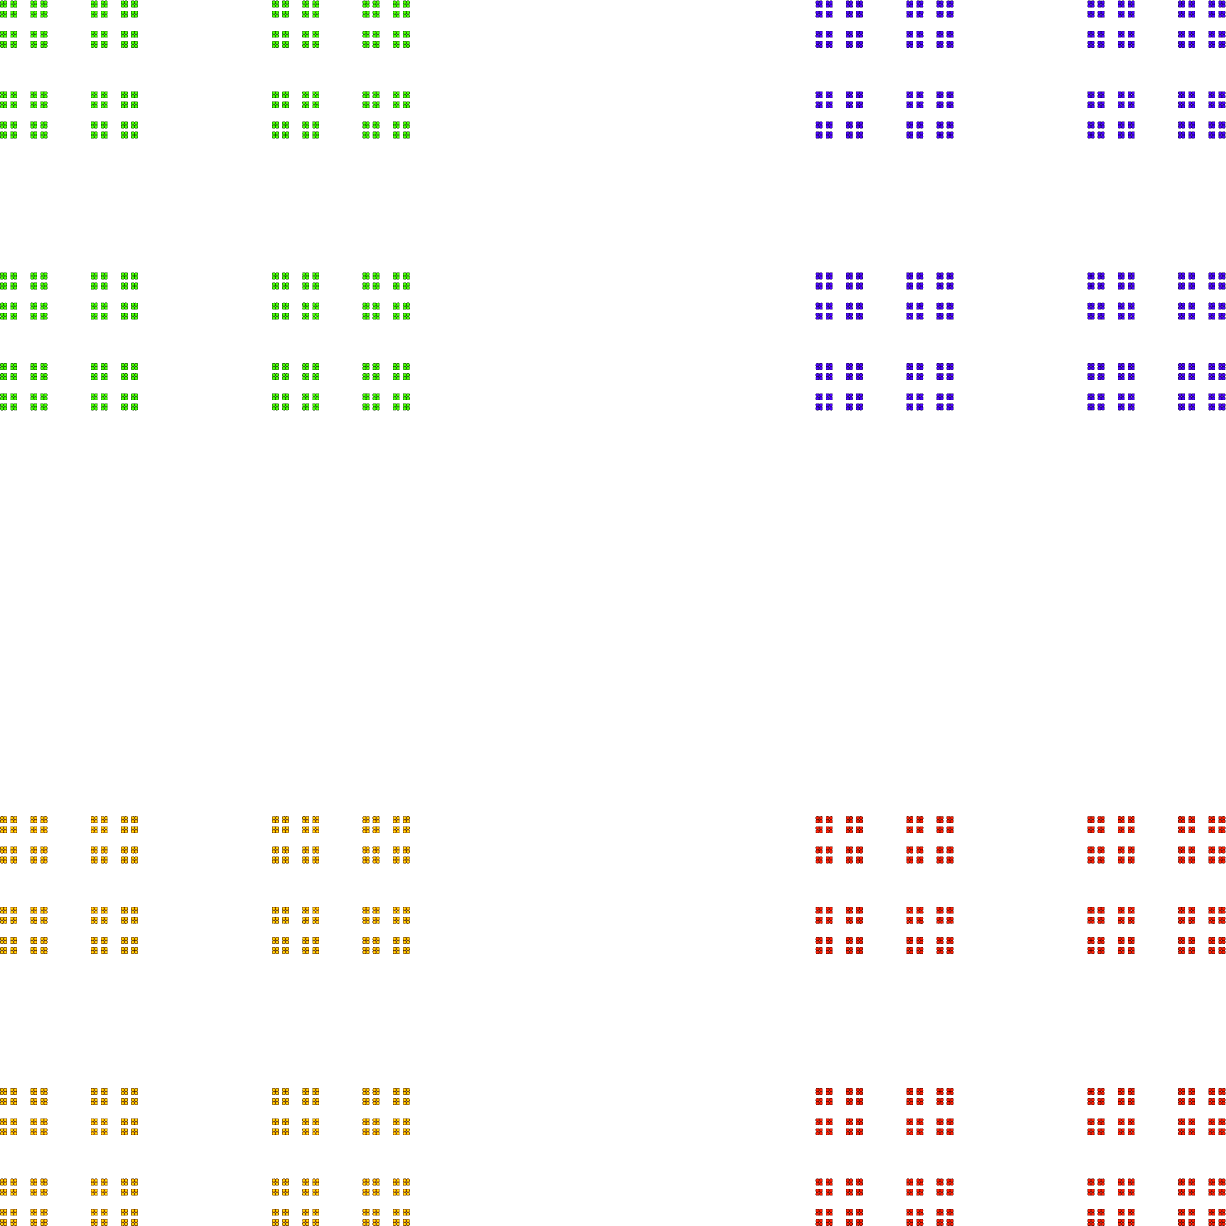
\includegraphics[width=0.3\textwidth]{CS.png}
\hfill
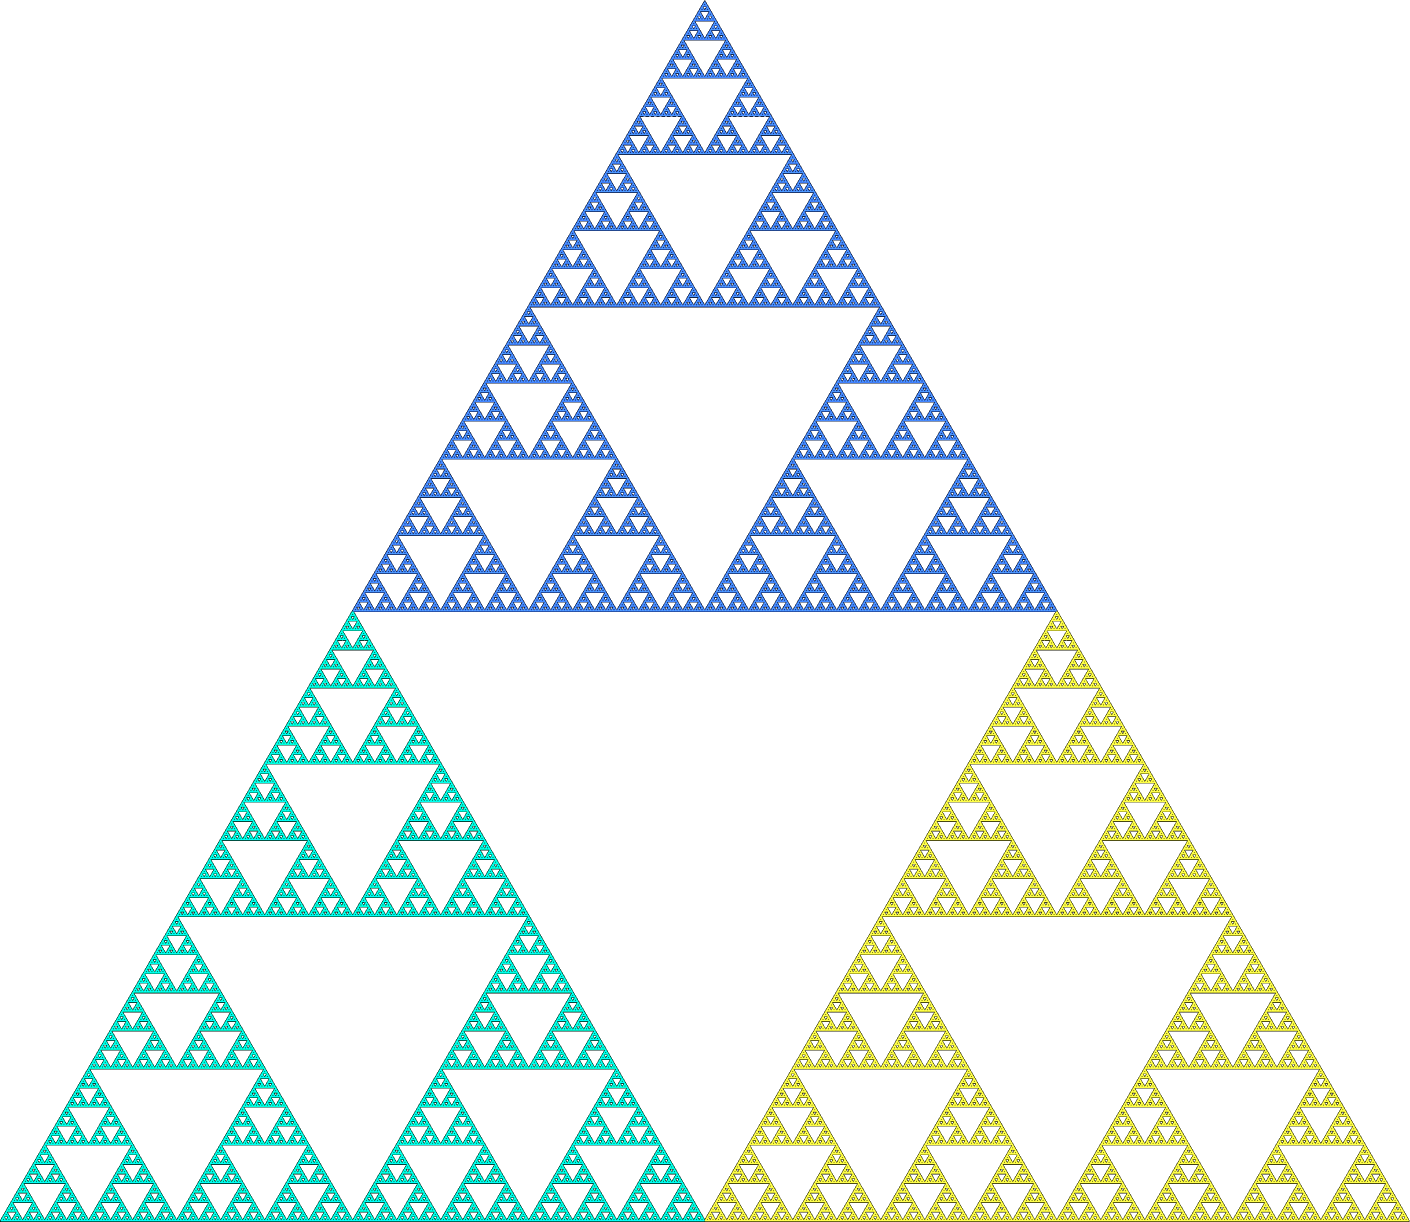
\includegraphics[width=0.3\textwidth]{SerpTri.png}
\hfill
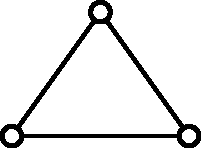
\includegraphics[width=0.3\textwidth]{SIG.pdf}
\caption{Вполне несвязное множество (слева), треугольник Серпинского и его граф пересечений.}
\end{figure}


\subsection{Критическое множество и самоподобная граница}

Пусть $\eC:=\{x:\; x\in S_i(K)\cap S_j(K),\; i,j \in I, i\neq j\}$ --- это объединение всех попарных пересечений $S_i(K)\cap S_j(K)$ (при $i\neq j$) копий первого порядка самоподобного множества $K$.
Назовём такое $\eC$ {\em критическим множеством}.

Тогда множество $\dd K:=\{x\in K: \text{ для некоторого }\bj\in I^* \text{ верно } S_\bj(x)\in C\}$ назовём {\em самоподобной границей} для $K$.
Говоря иначе, самоподобная граница $\dd K$ --- это множество всех предшественников точек из критического множества $\eC$.



{\em Посткритическое множество} (или {\em самоподобная граница}) $\eP$ системы $\eS$ --- это множество всех таких $\alpha\in I^{\8}$, что для некоторых ${\bf j}\in I^*$, $S_ {\bf j}(\alpha)\in\eC$. 
Другими словами, $\eP= \lbrace \sigma^k(\alpha) : \alpha\in \eC,k\in \mathbb{N}\rbrace$, где отображение $\sigma^k:I^{\8}\to I^{\8}$ определяется как $\sigma^k(\al_1\al_2\ldots)=\al_{k+1}\al_{k+2}\ldots$

Система $\eS$ называется {\em посткритически конечной} \cite{Kig}, если её посткритическое множество $\eP$ конечно. 
Таким образом, если система $\eS$ посткритически конечна, то существует конечное множество $\eV=\pi(\eP)$ такое, что для любых несравнимых $\bi,\bj\in\ia$,  $K_\bi\cap K_\bj= S_\bi(\eV)\cap S_\bj(\eV)$.\\

\begin{example}
Рассмотрим самоподобный дендрит со следующего Рисунка и отметим синим цветом точки критического множества и красным самоподобную границу.
\begin{figure}[H]
\centering
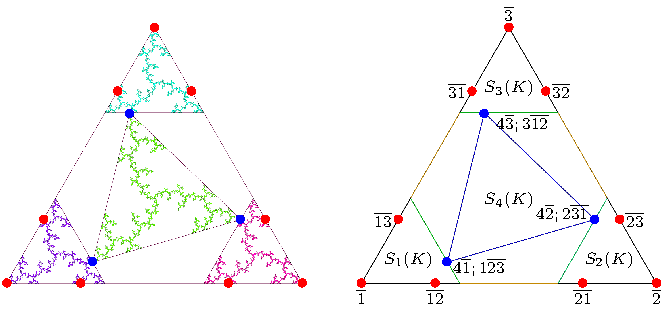
\includegraphics[width=\textwidth]{tr9.pdf}
\caption{Самоподобный дендрит, его критическое множество и самоподобная граница.}
\end{figure}
Каждая точка критического множества имеет по два адреса.
В данном примере все адреса точек критического множества периодические, поэтому посткритическое множество конечно (а значит конечна и самоподобная граница).

Обозначим точки $x=\pi(4\overline{1})=\pi(1\overline{23})$, $y=\pi(4\overline{2})=\pi(2\overline{31})$ и $z=\pi(4\overline{3})=\pi(3\overline{12})$.
Самоподобную границу будут образовывать последовательности предшественников этих трёх точек по каждому адресу.
Так у $x$ предшественниками будут точки $\pi(\overline{1})$, $\pi(\overline{23})$ и $\pi(\overline{32}).$
У $y$ предшественниками будут точки $\pi(\overline{2})$, $\pi(\overline{31})$ и $\pi(\overline{13}).$
И, соответственно у точки $z$ предшественниками будут точки $\pi(\overline{12})$, $\pi(\overline{21})$ и $\pi(\overline{3})$.
\end{example}

\subsection{Дендрит}

На протяжении всей работы, а особенно в текущей Главе, особый интерес для меня будут представлять самоподобные множества, являющиеся денритами. 

\begin{restatethis}{definition}{dfn:den} %\label{dfn:den}
{\em (К. Куратовский, \cite{Kur1}; J. Charatonik, W. Charatonik, \cite{Char1998})}
{\em Дендрит} --- это локально связный континуум, не содержащий простых замкнутых дуг.     
\end{restatethis}

Простая замкнутая дуга --- это непрерывный иньективный образ окружности.
Дедриты обладают некоторыми примечательными свойствами:
\begin{enumerate}[nolistsep]
\item[1.] Любые две точки дендрита можно соединить единственной лежащей в этом дендрите жордановой дугой;
\item[2.] Любое связное подмножество дендрита само является дендритом;
\item[3.] Пересечение любых связных подмножеств дендрита связно;
%\item[4.] ...
\end{enumerate}

Порядок ветвления $Ord(p,X)$ точки $p$ относительно дендрита $X$ --- это число компонент множества $X\setminus\{p\}$.
Точки порядка $1$ в дендрите $X$ называется {\em концами} в $X$; точки с порядком  $2$ называется {\em разбивающими точками}; точки же с порядком не менее $3$ называются {\em точками ветвления} в $X$.

Континуум $X$ будет дендритом тогда и только тогда, когда $X$ локально связно и  любые две точки соединяются единственной дугой. \\

Для простого графа пересечений и критерия связности не важно, по какому множеству пересекаются копии, важен сам факт того, что пересечение не пусто. 
Но в самоподобном дендрите пара копий пересекается либо по пустому, либо по связному множеству, то есть по поддендриту.
Удобнее же всего строить и изучать случаи с одноточечным пересечением.

\begin{definition}
Набор компактов $\eA=\{A_i,\ i\in I\}$ в $\mathbb{R}^n$ обладает {\em свойством одноточечного пересечения}, если для любых $i\neq j\in I$, пересечение $P_{ij}=A_i\cap A_j$ не более чем одноточечно.
\end{definition}

Мы можем определить наличие такого свойства у аттрактора системы сжимающих подобий следующим образом.
Пусть $\eS=\{S_1,\ldots ,S_m\}$ --- система сжимающих отображений в полном метрическом пространстве $X$, а $K$ --- её аттрактор. 
Пусть $\eA(\eS)=\{K_1,\ldots , K_m\}$. % и $\eA_n(\eS)=\{K_\bi:\bi\in I^n\}$.
Соответственно систему отображений $\eS$ будем называть {\em системой со свойством одноточечного пересечения}, если система $\eA(\eS)$ является системой множеств с одноточечным пересечением.

\begin{definition}
Пусть $K=K(\eS)$ --- самоподобное множество, обладающее свойством одноточечного пересечения.
{\em Граф пересечений} $\Gamma(\eS)$ системы $\eS$ --- это двудольный граф с долями $\eK=\{K_i:\; i\in I\}$ и $\eP=\{p:\;p\in K_i\cap K_j,\; i,j\in I, i\neq j\}$, и с множеством рёбер $E=\{(K_i,p):p\in K_i\}$.
\end{definition}

Иными словами, мы в графе первой доле (белым вершинам) ствим в соответсвие копию самоподобного множества, а второй доле (чёрным вершинам) мы ставим в соответствие все точки из попарных пересечений копий самоподобного множества.
Тогда мы соединяем ребром белую и чёрную вершину, если соответсвующая точка пересечения содержится в соответсвующей копии.

Преимущество двудольного графа пересечений перед простым графом пересечений состоит в том, что тройке копий, пересекающихся по одной точке, в первом графе соответствует подграф в форме дерева, в то время как во втором графе мы получаем цикл из трёх вершин.
Это особенно полезно для следующей теоремы, позволяющей проверить, является ли самоподобное множество дендритом.

\begin{theorem}[Tetenov A. V. (2021),см. {\cite[Th.1.7]{FPS}}]
\label{thm:fpden}
Пусть $K=K(\eS)$ --- самоподобный континуум со свойством одноточечного пересечения.
Если граф пересечений $\hat\Gamma(\eS)$ системы $\eS$ является деревом, то её аттрактор $K$ --- дендрит с одноточечным пересечением.
\end{theorem}

\begin{figure}[H]
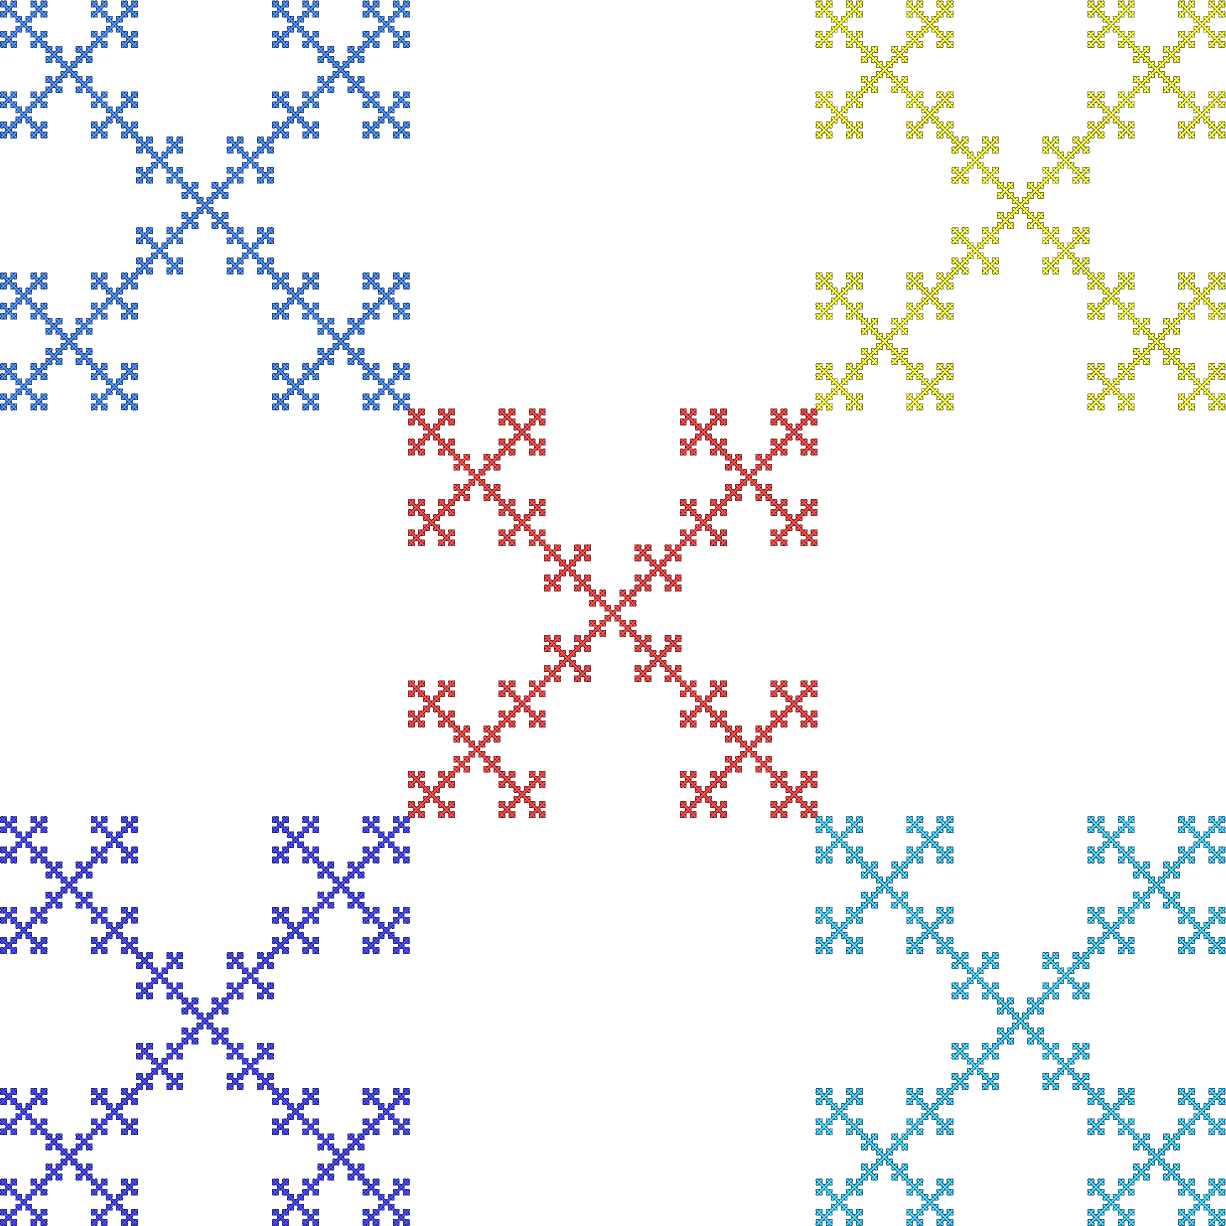
\includegraphics[width=0.4\textwidth]{VicsekSet.png}
\hfill
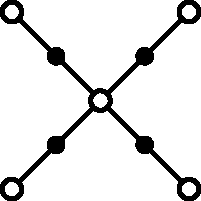
\includegraphics[width=0.4\textwidth]{BIG.pdf}
\caption{Самоподобный дендрит (слева) и его двудольный граф пересечений (справа).}
\end{figure}

Именно такие самоподобные дендриты с одноточечным пересечением мы и будем рассматривать в текущей Главе.  
И первым удобно задаваемым классом самоподобных дендритов с одноточечным пересечением являются аттракторы полигональных систем.

\subsection{Стягиваемые полигональные системы}

Самюэль М., Тетенов А. В. и Ваулин Д. А. в своей работе \cite{STV2017} рассматривают самоподобные дендриты, являющиеся аттракторами стягиваемых полигональных систем, которые задаются следующим образом.

\red{Пусть также $\Om(P,A)$ обозначает угол при вершине $A$ в многоугольнике $P$.}
% используется после вторго параграфа, надо перенести туда

\begin{restatethis}{definition}{dfn:cps} \label{dfn:cps}
Пусть $P\subset\mathbb{R}^2$ --- это ограниченный многоугольник гомеоморфный диску, а $ \eV_P= \{A_1, \ldots, A_{n_P}\}$ --- множество его вершин.
Пусть дана система подобий $\eS = \{S_1, \ldots, S_m\}$ в ${\mathbb{R}}^2$ такая, что:
\begin{itemize}[nolistsep]
\item[{\bf (D1)}] для любого $i \in I$ множество $P_i = S_i (P) \subset P$; 
\item[{\bf (D2)}] для любого $i \ne j, i, j \in I, P_i \bigcap P_j =  \eV_{P_i} \bigcap  \eV_{P_j}$ и $\#(\eV_{P_i} \bigcap  \eV_{P_j})<2$;  
\item[{\bf (D3)}] $\eV_P \subset \bigcup \limits_{i \in I} S_i (\eV_P)$;
\item[{\bf (D4)}] множество $\widetilde P = \bigcup \limits_{i = 1} ^m P_i$ стягиваемо.
\end{itemize} 
Такая система  $\eS$, удовлетворяющая условиям $\bf (D1 - D4)$, называется  {\em стягиваемой $P$-полигональной системой подобий}.
\end{restatethis}

\begin{figure}[H]
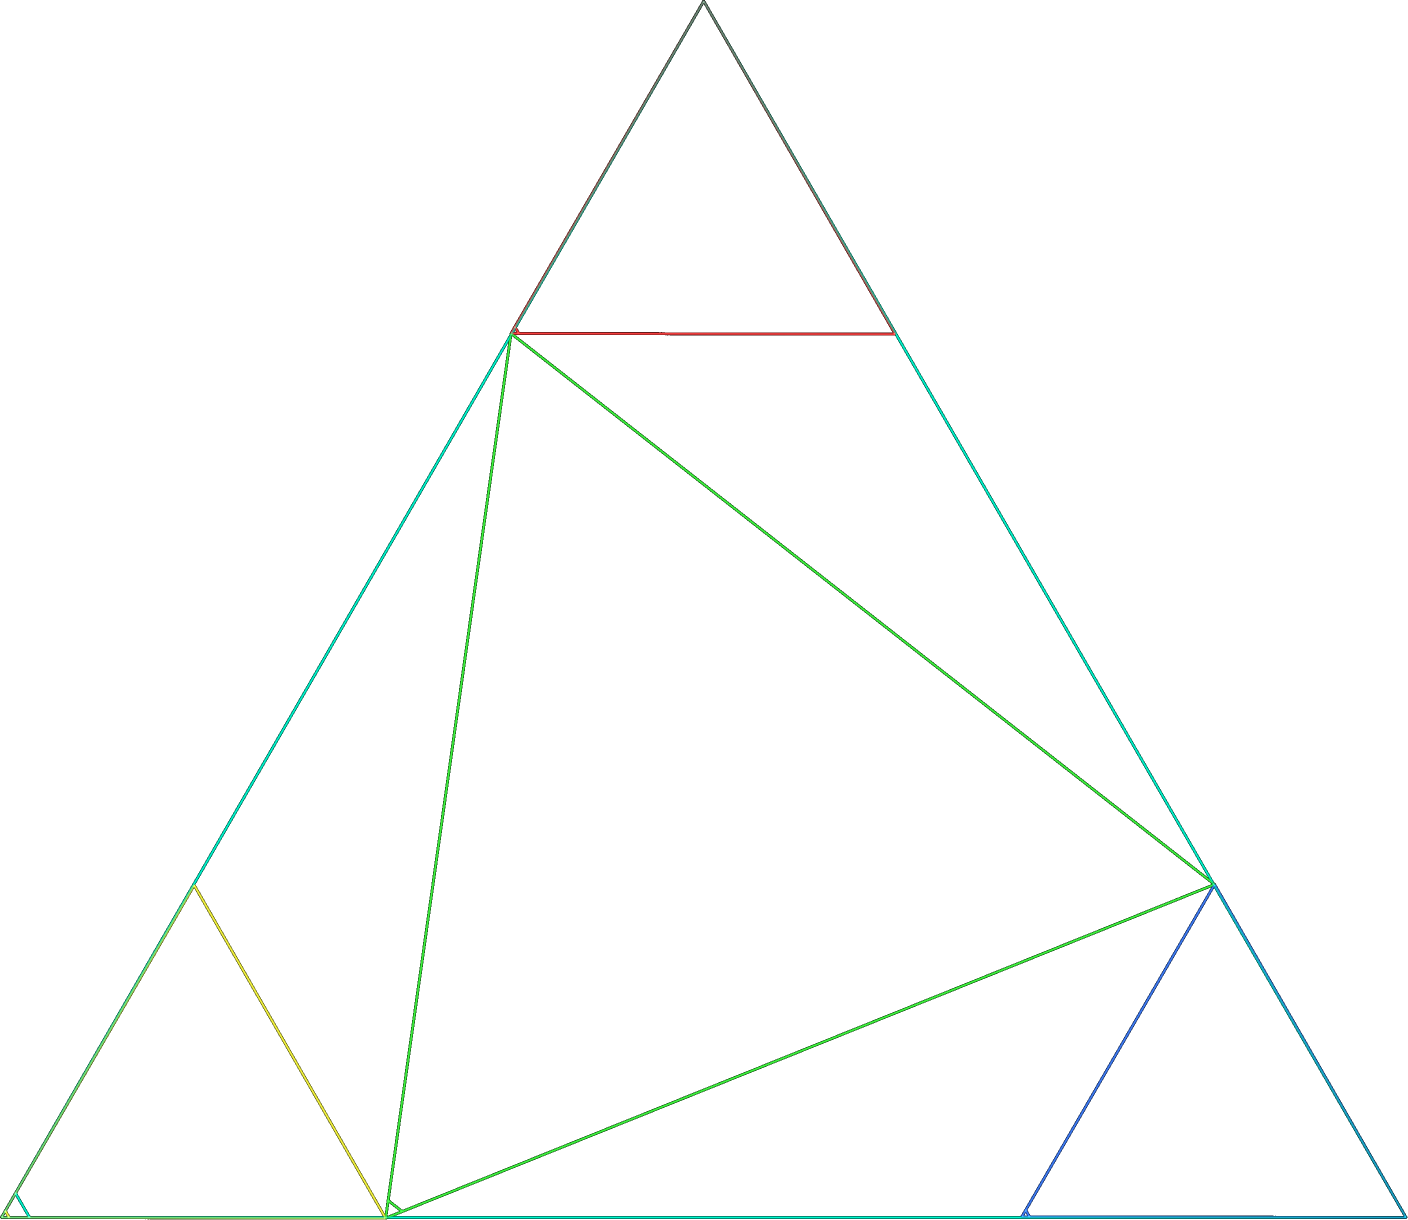
\includegraphics[width=0.45\textwidth]{CPS1_P.png}
\hfill
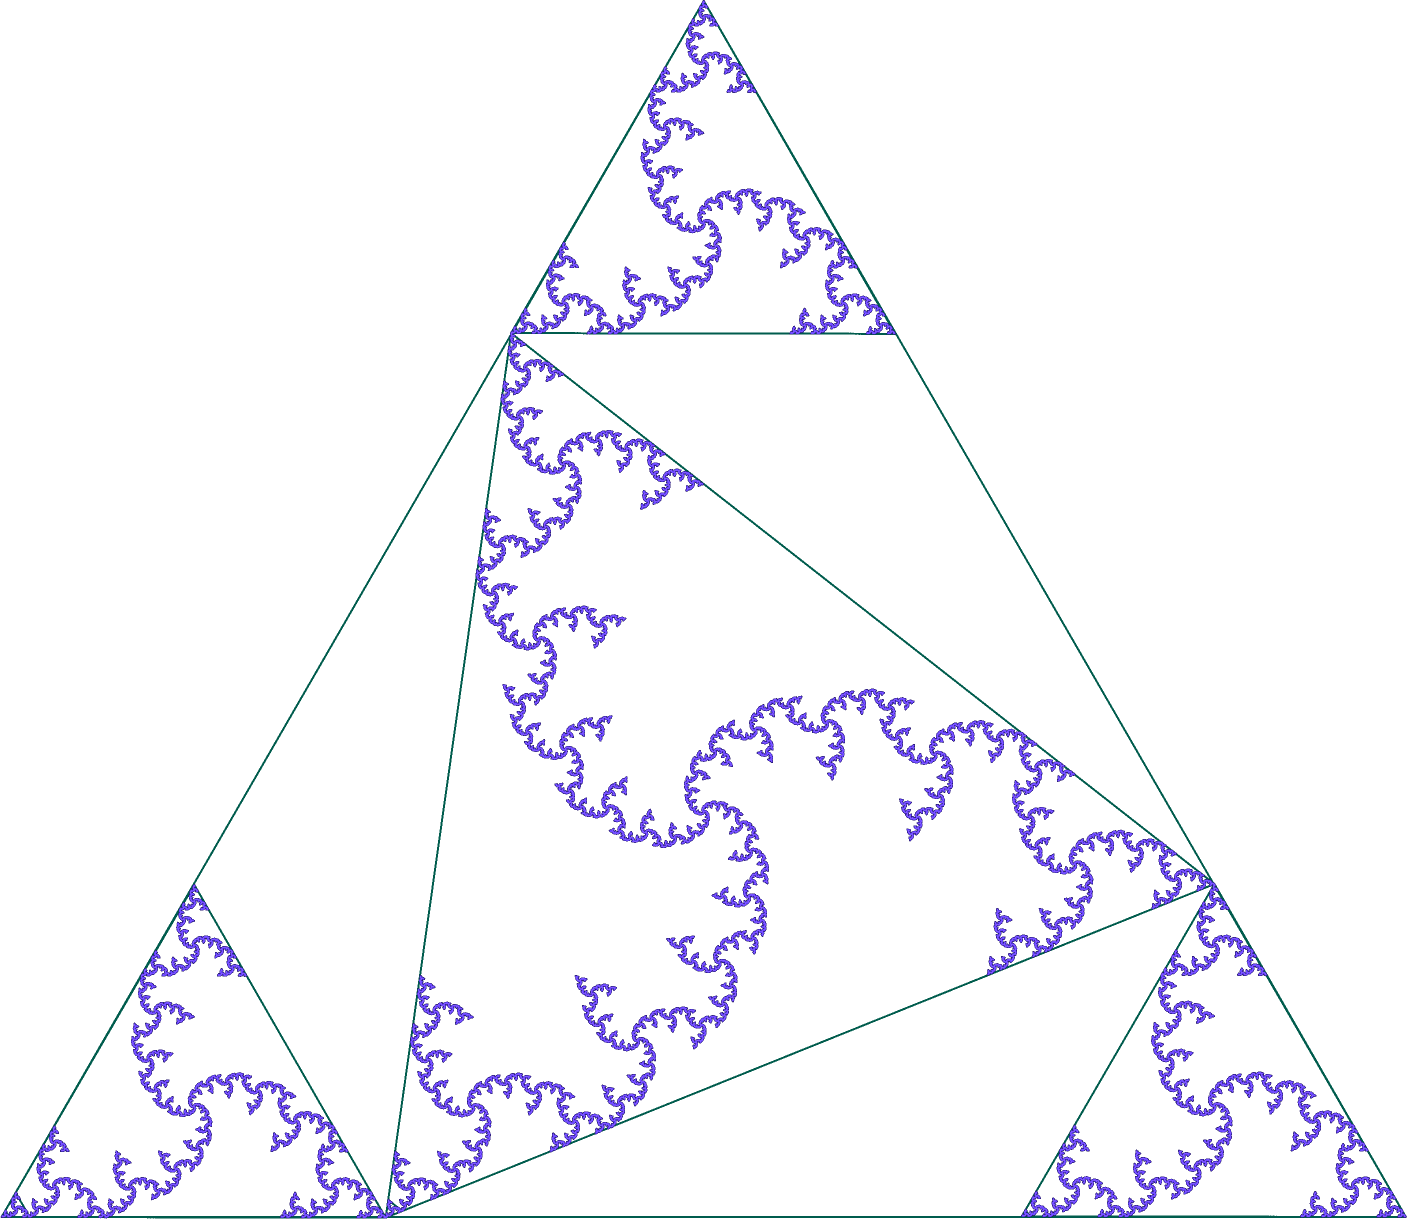
\includegraphics[width=0.45\textwidth]{CPS1_K.png}
\caption{Система многоугольников, задающая полигональную систему $\eS$ (слева), и аттрактор $K(\eS)$ этой системы (справа).}
\end{figure}

\begin{restatethis}{theorem}{thm:cpsden} %\label{thm:cpsden} 
Аттрактор $K$  стягиваемой  $P$-полигональной системы подобий $\eS$ является дендритом.
\end{restatethis}

Это действительно так, ведь из условий следует, что $K\IN P$, а значит $K_i\cap K_j=P_i\cap P_j$.
Значит у аттрактор полигональной системы --- множество с одноточечным пересечением, двудольный граф пересечения которого является деревом.
Значит, согласно Теореме \ref{thm:fpden}, этот аттрактор является дендритом с одноточечным пересечением.\\

Авторами в \cite[Theorem 4]{TSV2017} было показано, что
\begin{enumerate}[nolistsep]
\item[1.] Всякая стягиваемая полигональная система удовлетворяет (OSC), где  в качестве открытого множества мы можем взять $\dot P$;
\item[2.] $P_\bj\IN P_\bi$ тогда и только тогда, когда  $\bj\sqsupset\bi$, а если $\bi\sqsubset\bj$, то  $ S_\bi(\eV_P)\cap P_\bj\IN S_\bj(\eV_P)$;
\item[3.] Если $\bi,\bj\in \ia$ несравнимы, то $P_\bi\cap P_\bj$ либо пусто, либо является  общей вершиной многоугольников $P_\bi$ и  $P_\bj$;
\item[4.] При этом все вершины $P$ лежат в $K$, поэтому и множество $G_\eS(\eV_P)$ вершин многогранников $P_\bj$ содержится в $K$ и плотно в $K$, а всякая точка $x\in K\mmm G_\eS(\eV_P)$ имеет единственный адрес.
\end{enumerate}
 
В первой Главе я получаю и рассматриваю обобщение таких полигональных систем.
 

% \resizebox{.9    \textwidth}{!}{{
% \begin{tikzpicture}[line cap=round,line join=round,>=stealth ,scale=1]\scriptsize
% \node at (-6.3,-2.3) {
%   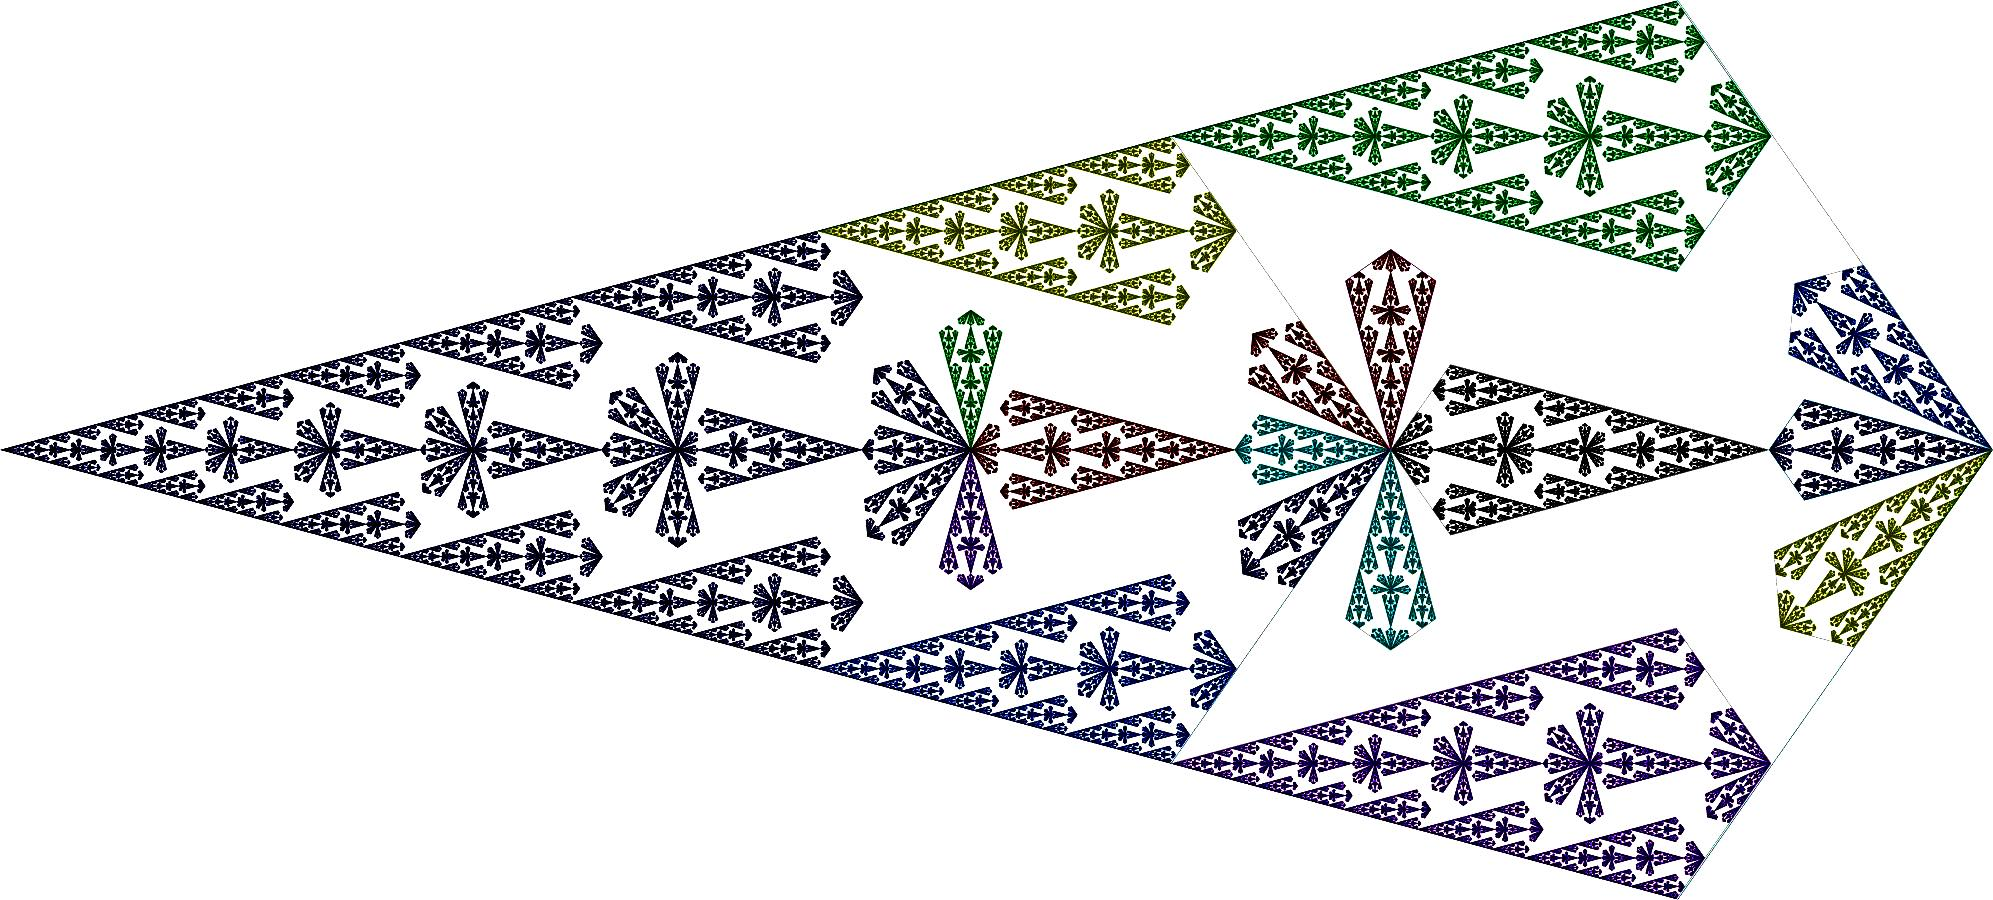
\includegraphics[width=.57\textwidth]{Krpt.jpg}}; \node at (2,-2) {\includegraphics[width=.35\textwidth]{trucs.jpg}};

% %\draw[step=.1,lightgray,ultra thin] (-11,-5) grid (5,0);
%   %\draw[step=.2,yellow,ultra thin] (-11,-5) grid (6,0);
%   %\draw[step=1,green, thin] (-11,-5) grid (5,0);
%   \node at(-5.3,-.25){$B$}; \node at (-8.5,-4) {\small Полигональная система и ее аттрактор};\node at (2,-4) {\small Локальная структура  $K$ около вершины $B$.(повернуто)};\node at (-4.15,-3.35) {$\scriptsize{\rho_0}$};
% \path[thick,red]
% 	   (-5.3,-.4) edge[->]  (-4.44,-2.2);
% 	   \path[thin,red] (-4.38,-3.27) edge[<->]  (-4.3,-3.5);
% 	   %\path[thick,red] (-3,-0.12) edge[]  (-1.47,-2.3);
% \end{tikzpicture}}} 

%%%%%%%%%%%%%%%%%%%%%%%%%%%%%%%%%%%%%%%%%%%%%%%
\section{Обобщенные полигональные системы.} 

%\subsection{Системы с одноточечным пересечением и граф пересечений}
%
%При рассмотрении обобщенных полигональных систем мы будем опираться на ряд определений и утверждений из работы Тетенова А. В. \cite{FPS}.
%
%\begin{definition}\label{fipss}
%Пусть $\eA=\{A_i,i\in I\}$ -- конечная система компактных множеств такая, что для любых $i\neq j\in I$, $\# A_i\cap A_j \le 1$. 
%Тогда $\eA$ --- система множеств с одноточечным пересечением.
%\end{definition}
% 
%Пусть $P$ --- множество точек попарного пересечения множеств $A_i$, а $P_i=A_i\cap P$.
%
%\begin{definition}\label{igraph}
%Граф пересечений  $\Ga(\eA)$ системы множеств  $\eA$ с одноточечным пересечением --- это двудольный граф  $(P,\eA; E)$, для которого  $e=\{A_i,p\}\in E$ тогда и только тогда, когда $p\in A_i$. 
%\end{definition}
%
%Мы называем $A_i\in \eA$ {\em белыми вершинами} , а $p\in P$ --- {\em черными вершинами}.  
%Множество $N(A_i)$ черных вершин, смежных к белой вершине $A_i$ совпадает с $P_i$, тогда как для черной вершины $p$,  $N(p)=\{A_i:p\in A_i\}$. 
%Поскольку $p$ является точкой пересечения по крайней мере двух множеств $A_i$, то $ \mathrm{deg}(p)\ge 2$.
% 
%Определения \ref{fipss} и \ref{igraph}  мы можем применить к системам сжимающих отображений и их аттракторам.
%
%Пусть $\eS=\{S_1,\ldots ,S_m\}$ --- система сжимающих отображений в полном метрическом пространстве $X$, а $K$ --- её аттрактор. 
%Пусть $\eA(\eS)=\{K_1,\ldots , K_m\}$ и $\eA_n(\eS)=\{K_\bi:\bi\in I^n\}$.
%
%\begin{figure}[H]
%    \centering
%    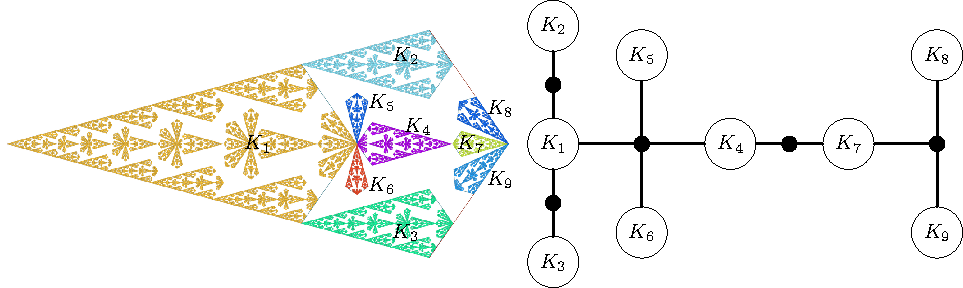
\includegraphics[width=\textwidth]{PS_and_IG.pdf}
%    % \includestandalone[width=\textwidth]{images/tikz1/PS_and_IG.tex}
%    \caption{Полигональная система и её граф пересечений}
%    \label{img:exgp1}
%\end{figure}
% 
%\begin{definition}\label{fipcs}
%Систему отображений $\eS$ будем называть {\em системой со свойством одноточечного пересечения}, если система $\eA(\eS)$ является системой множеств с одноточечным пересечением.
%\end{definition}
%
%\begin{theorem}{\em (см. \cite[Th.1.7]{FPS})} \label{fpden}
%Пусть $\eS$ --- система сжимающих отображений со свойством одноточечного пересечения, граф пересечений которой является деревом. 
%Тогда ее аттрактор $K$ --- дендрит.
%\end{theorem}



\subsection{Обобщенные полигональные системы}



Если мы опустим условие {\bf(D1)} в Определении \ref{dfn:cps} стягиваемой $P$-полигональной системы $\eS$, то получим определение {\em обобщенной $P$-полигональной системы}:

\begin{restatethis}{definition}{dfn:gps} \label{dfn:gps}
Система $\eS=\{S_1,\ldots ,S_m\} $, удовлетворяющая условиям {\bf D2-D4} Определения \ref{dfn:cps}, называется обобщенной $P$-полигональной системой подобий.    
\end{restatethis}

\begin{figure}[H]
    \centering
    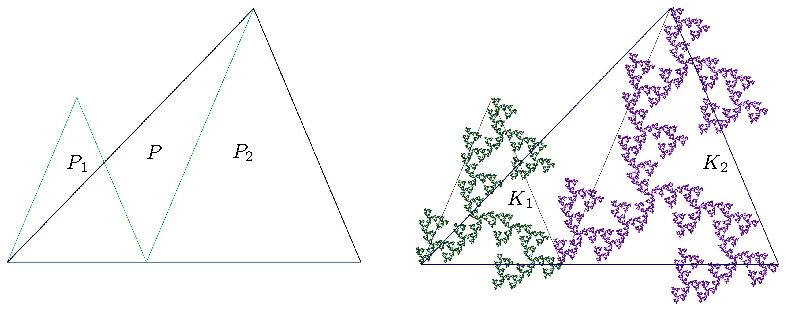
\includegraphics[width=\textwidth]{GPS_and_A.pdf}
    % \includestandalone[width=\textwidth]{images/tikz1/GPS_and_A.tex}
    \caption{Обобщенная полигональная система и её аттрактор}
    \label{img:ops}
\end{figure}

Для таких систем не обязано выполняться включение $S_i(P)\IN P$.
И хотя аттрактор такой системы будет связен, но дендритом он уже может и не быть, поскольку пересечение копий может быть неодноточечным:
$$S_i(K)\cap S_j(K)\supseteq S_i(P)\cap S_j(P).$$
Тем не менее, если это включение станет равенством, то это будет означать, что $\eS$ --- система с одноточечным пересеченьем, а значит её аттрактор имеет двудольный граф пересечений в форме дерева и является дендритом.



\begin{restatethis}{theorem}{thm:pcint}\label{thm:pcint}
Пусть $\eS$ --- обобщенная $P$-полигональная система.  
Если для любых $i, j \in I$ 
\begin{equation}\label{icnd}
S_i(K)\cap S_j(K)=P_i\cap P_j,
\end{equation} 
то 
\begin{itemize}[nolistsep]
    \item[(i)] аттрактор $K$ системы $\eS$ является дендритом;
    \item[(ii)] система $\eS$ удовлетворяет OSC;
    \item[(iii)] множество адресов $\pi^{-1}(x)$ всякой точки $x\in K$ конечно.
    % (iv) система $\eS$ посткритически конечна. 
\end{itemize}
   
\end{restatethis}


%\begin{remark}\label{fpro} 
%Если $\eS$ удовлетворяет условию \eqref{icnd}, то $\eS$ --- система с одноточечным пересечением, аттрактор $K$ которой связен, а самоподобная граница $\dd K=\eV_P$. 
%\red{Свойства таких систем разобраны в \cite{FPS}.}
%В этом случае для любых не сравнимых мультииндексов $\bi,\bj\in \ia$, пересечение $K_\bi\cap K_\bj=S_\bi(\eV_P)\cap S_\bj(\eV_P)$ либо пустое либо одноточечное.
%\end{remark}

\begin{proof}
(i) Действительно, из формулы (\ref{icnd}) следует, что графы пересечений $\Ga(\{K_i\})$ и $\Ga(\{P_i\})$ совпадают. 
Из свойств {\bf (D2)-(D4)} следует, что граф пересечений обобщенной полигональной системы  $\Ga(\{P_i\})$ --- дерево. 
Из Теоремы \ref{fpden} следует, что $K$ --- дендрит.

(ii) Выполнение условия открытого множества (OSC) для систем $\eS$ сжимающих подобий в $\rr^2$ с конечным пересечением и связным аттрактором $K$ доказано в \cite{BR}.

(iii) Конечность множества $\pi^{-1}(x)$ следует из \cite[Proposition 2.3]{FPS}.
\end{proof}




\begin{remark}\label{n1pi}  
Обобщенная $P$-полигональная система $\eS$ может не удовлетворять условию \ref{icnd} и иметь аттрактор $K$, являющийся дендритом. 
Аттрактор $K$ обобщенной полигональной системы $\eS$ на Рисунке ниже является дендритом, но  $P_7\cap P_9=\0$, тогда как $K_7\cap K_9$ -- это отрезок.
\end{remark}

\begin{figure}[H]
    \centering
    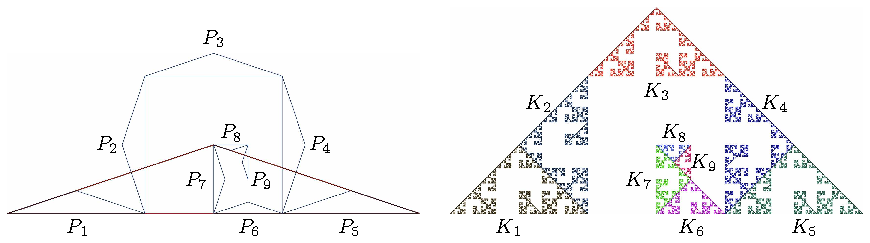
\includegraphics[width=\textwidth]{example_rmk2.pdf}
    % \includestandalone[width=\textwidth]{images/tikz1/example_rmk2.tex}
    \caption{Пример к замечанию \ref{n1pi}}
\label{img:rmk1}
\end{figure}

\begin{corollary}
%Let $\eS$ be a generalized $P$-polygonal system, satisfying the condition(\ref{icnd}). For any subarc $\ga_{xy}\IN K$ and for any $n$, there is a unique chain of pairwise different multiindices $\bi_1,\bi_2,\ldots ,\bi_l\in I^n$, which divides $\ga_{xy}$ to sequential arcs $\ga_{xx_1}\IN K_{i_1},\ldots,\ \ga_{x_{k-1}x_k}\IN K_{i_k},\ldots,\ \ga_{x_{l-1}y}\IN K_{i_l}$.\qed
Пусть $\eS$ -- обобщенная $P$-полигональная система, удовлетворяющая условию (\ref{icnd}). Для любой поддуги $\ga_{xy}\IN K$ и для любого $n$ существует единственная цепочка попарно различных мультииндексов $\bi_1,\bi_2,...,\bi_l\in I^n$, которая разбивает $\ga_{xy}$ на последовательные поддуги $\ga_{xx_1}\IN K_{i_1},\ldots,\ \ga_{x_{k-1}x_k}\IN K_{i_k},\ldots,\ \ga_{x_{l-1}y}\IN K_{i_l}$.\qed
\end{corollary}


\subsection{$\da$-деформации стягиваемых полигональных систем.}
\begin{restatethis}{definition}{dfn:deform}\label{dfn:deform} 
Пусть $\da>0$. Обобщенная $P'$-полигональная система $\eS'=\{S'_1,...,S'_m\}$ называется $\da$-деформацией $P$-полигональной системы $\eS=\{S_1,...,S_m\}$, если существует биекция $f:\bigcup\limits_{k=1}^m \eV_{P_k}\to \bigcup\limits_{k=1}^m \eV_{P'_k}$ такая, что
\begin{itemize}[nolistsep]
    \item[a)] $f|_{\eV_P}$ продолжается до гомеоморфизма $\tilde f: P\to  P'$;
    \item[b)] $|f(x)-x|<\delta$  для любого $x\in \bigcup\limits_{k=1}^m \eV_{P_k}$;
    \item[c)] $f(S_k(x))=S'_k(f(x))$ для любого $k\in I$ и $x\in \eV_P$.
\end{itemize}    
\end{restatethis}


\begin{figure}[H]
    \centering
    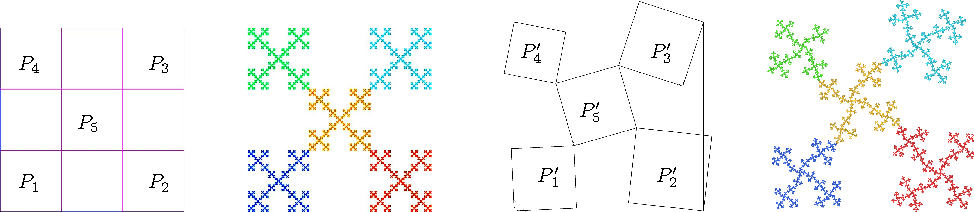
\includegraphics[width=\textwidth]{PS_and_deltadef.pdf}
    % \includestandalone[width=\textwidth]{images/tikz1/PS_and_deltadef.tex}
    \caption{Полигональная система $\eS$ и её $\da$-деформация $\eS'$ }
    \label{img:ddef}
\end{figure}

Поскольку $\hat f$ --- гомеоморфизм многоугольников, переводящий вершины в вершины, мы можем предполагать, что $\hat f$ является симплициальным изоморфизмом некоторой триангуляции $P$ с вершинами в $V_P$ на эквивалентную ей триангуляцию $P'$ c вершинами в $V_{P'}$.\\ 
 
По условию c), если  $i,j\in I$, $A_1,A_2\in \eV_P$ и $S_i(A_1)=S_j(A_2)$, то $S'_i( f(A_1))=S'_j(f(A_2))$.\\  Такое же соотношение выполняется и в случае, если $\bi,\bj\in \ia$ --- мультииндексы:

\begin{lemma}\label{bibj}
Если $A_1,A_2\in \eV_P$, $\bi,\bj\in\ia$ и $S_\bi(A_1)=S_\bj(A_2)$, то $S'_\bi( f(A_1))=S'_\bj( f(A_2))$.
\end{lemma}
 
\begin{proof}
Предположим, что $S_\bi(A)=B\in \eV_\wP$ для некоторого $A\in \eV_P$, и пусть $\bi=i_1i_2...i_n$. 
Обозначим $S_{i_{k+1}...i_n}(A)$ как $A_k$.

Тогда мы имеем конечную последовательность соотношений между $B\in \eV_\wP$ и вершинами $A_k\in\eV_P$:\\
\begin{equation}\label{chn1}
B=S_{i_1}(A_1); \quad A_1=S_{i_2}(A_2); \quad \ldots A_{n-1}=S_{i_n}(A)
\end{equation}
По условию c),  отображение $f$ преобразует  эти соотношения  в  
\begin{equation}\label{chn2} 
B'=S'_{i_1}(A'_1); \quad A'_1=S'_{i_2}(A'_2); \quad \ldots  A'_{n-1}=S'_{i_n}(A'), 
\end{equation}
поэтому $S'_\bi(A')=B'$ и, если $S_\bi(A_1)=S_\bj(A_2)\in \eV_{\wP}$, то $S'_\bi(f(A_1))=S'_\bj(f(A_2))$.

Теперь предположим,  что $S_\bi(A_1)=S_\bj(A_2)$ и $\bi=\bl\bi'$, $\bj=\bl\bj'$ и $S_\bi(A_1)=S_\bj(A_2)=S_\bl(B)$ для некоторого $B\in \eV_\wP$. 
Тогда  $S_{\bi'}(A_1)=S_{\bj'}(A_2)=B$, следовательно $S'_{\bi'}(f(A_1))=S'_{\bj'}(f(A_2))=f(B)$ и
$S'_{\bi}(f(A_1))=S'_{\bj}(f(A_2))=S'_\bl(f(B))$.
\end{proof}

\begin{restatethis}{theorem}{thm:attrmap}\label{thm:attrmap}
Пусть  $\da$-деформация $\eS'$ стягиваемой $P$-полигональной системы $\eS$ задается биекцией $f:\bigcup\limits_{k=1}^m \eV_{P_k}\to \bigcup\limits_{k=1}^m \eV_{P'_k}$, а $\pi:I^\8\to K, \pi':I^\8\to K'$ --- индексные отображения этих систем.
\begin{itemize}[nolistsep]
    \item[(i)] $f$ однозначно задает непрерывное продолжение $\hat f:K\to K'$ такое, что $\hat f\circ\pi=\pi'$.
    \item[(ii)] Если $\eS'$ удовлетворяет условию \eqref{icnd}, то $\hat f$ является гомеоморфизмом.
\end{itemize}    
\end{restatethis}

\begin{remark}
Равенство  $\hat f\circ\pi=\pi'$ эквивалентно тому, что для любого $z\in K$ и $\bi\in\ia$,
\begin{equation}\label{compat}
\hat f(S_\bi(z))=S'_\bi(\hat f(z)).
\end{equation}
\end{remark}

\begin{proof}
Доказательство аналогично (см.\cite[Lemma 1.]{ATK}). 
Во-первых, мы определим функцию $\hat f$, которая является сюрьекцией плотного подмножества $G_\eS(\eV_P)\IN K$ в плотное подмножество $G_{\eS'}(\eV_{P'})\IN K'$. 
Во-вторых, мы покажем, что она непрерывна по Гёльдеру на $G_\eS(\eV_P)$, и, следовательно, имеет единственное непрерывное продолжение до сюрьекции из $K$ в $K'$, которое мы обозначим для прежднего символа как $\hat f$. 
В-третьих, мы покажем, что условие \ref{icnd} подразумевает, что $\hat f$ является инъективным и поэтому является гомеоморфизмом..\\

1. Определим отображение $\hat f(z):G_\eS(\eV_P)\to G_{\eS'}(\eV_{P'})$ как
\begin{equation}\label{hatf}
\hat f(z)=S'_\bi(f(S_\bi^{-1}(z))\mbox{,  где   }z\in S_\bi(\eV_P).
\end{equation}

Как следует из Леммы \ref{bibj}, если $S_\bi(A_1)=S_\bj(A_2)=z$, то $S'_\bi(f(S_\bi^{-1}(z)))=S'_\bj(f(S_\bj^{-1}(z)))$, поэтому отображение $\hat f$ корректно определено. 

Очевидно, что $\hat f(G_\eS(\eV_P))= G_{\eS'}(\eV_{P'})$, потому что если $A'\in \eV_{P'}$ и $z'=S'_\bi(A')$, то существует вершина $A=f^{-1}(A')\in \eV_P$, вследствие этого $z'=\hat f(S_\bi(A))$.

Кроме того, для любого  $z\in G_\eS(\eV_P)$ и $\bi\in\ia$, $\hat f(S_\bi(z))=S'_\bi(\hat f(z))$ и если $z_1,z_2\in G_\eS(\eV_P)$, $\bi,\bj\in\ia$ и $S_\bi(z_1)=S_\bj(z_2)$, то $S'_\bi(\hat f(z_1))=S'_\bj(\hat f(z_2))$.\\

2. Пусть $q_k = \Lip S_k$, $q_k' = \Lip S_k'$,  $\beta = \min \limits _{k\in I } {\dfrac {\log {q'_k}} {\log {q_k}}}$.

Затем, следуя доказательству \cite[Теорема 27, step 4.]{TSV0}, в котором для наших оценок мы используем $K'$ вместо $P'$, мы видим, что для любых $z_1,z_2\in G_\eS(\eV_P)$,
$$|z_1'-z_2'| \le\dfrac {2|K'|} {(\rho_0\cdot\sin {(\al_0/2)})^{\beta}}|z_1-z_2|^{\beta}.$$
   
Поэтому отображение $\hat f$ может быть расширено до непрерывного по Гёльдеру сюрьективного отображения множества $K$ в $K'$. Поскольку для любого $z\in K$ и любого $k\in I$ справедливо $\hat f(S_k(z))=S'_k(f(z))$, то $\hat f\circ\pi=\pi'$.\\
 
3. Теперь предположим, что система $\eS'$ удовлетворяет условию (\ref{icnd}). 
Предположим, что для некоторых $\bm\sa=i_1i_2...\in I^\8$ и $\bm\tau=j_1j_2...\in I^\8$ справедливо $\hat f\circ\pi(\bm\sa)=\hat f\circ\pi(\bm\tau)$. Тогда, если $i_1\neq j_1$, то, по условию \ref{icnd}, $P'_{i_1}\cap P'_{j_1}\neq\0$, в результате чего   $P_{i_1}\cap P_{j_1}=\{B\}$ для некоторого $B\in \eV_\wP$ и $\pi(\bm\sa)=\pi(\bm\tau)=B$.
 
Пусть теперь  $\bm\sa=\bl\bm\sa'$ и $\bm\tau=\bl\bm\tau'$, а $\hat f\circ\pi(\bm\sa)=\hat f\circ\pi(\bm\tau)$. Тогда, по формуле \ref{compat}, $\hat f\circ\pi(\bm\sa')=\hat f\circ\pi(\bm\tau')$, так что если первые индексы в $\bm\sa'$ и  $\bm\tau'$ различны, то $\pi(\bm\sa)=\pi(\bm\tau)=S_\bl(B)$ для некоторого $B\in \eV_\wP$. 
 
Это подразумевает инъективность отображения $\hat f$. Таким образом $\hat f$ -- гомеоморфизм компактных множеств $K$ и $K'$.   
\end{proof}
 


\section{Теорема о совпадении параметров.}

\subsection{Циклические вершины и индексная диаграмма}

\begin{definition}\label{cyclic}
Пусть $\eS=\{S_i, i\in I\}$ --- обобщенная $P$-полигональная система. Индексной диаграммой системы $\eS$ называют ориентированный отмеченный мультиграф $\Ga=(V_P,E,\mu)$, где $V_P$ -- множество вершин многоугольника $P$, ребро $e\in E$ направлено из $A$ в $B$, если существует $S_i: S_i(B)=A$, при этом отображение $\mu:E\to I$ сопоставляет ребру  $e$  индекс  $\mu(e)=i$.
\end{definition}

Мы используем следующие обозначения для ребер в направленных графах: если $e$ -- ребро в графе $\Ga$,  направленное из $A$ в $B$, то $\al(e)=A$ и $\om(e)=B$. Путем $\sa$ в $\Ga$ называется последовательность ребер $e_1, e_2, ... e_n$ такая что $\al(e_k)=\om(e_{k-1})$ для всех $k>1$. $\al(\sa)=\al(e_1)$ и, если путь заканчивается ребром $e_n$, $\om(\sa)=\om(e_n)$.\\

\begin{figure}[H]
    \centering
    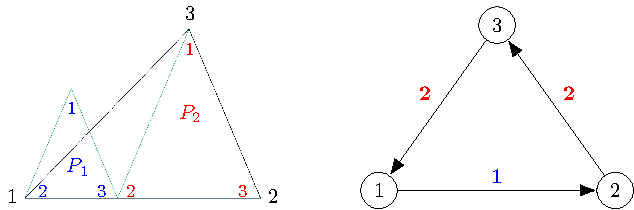
\includegraphics[width=0.7\textwidth]{id1.pdf}
    % \includestandalone[width=0.7\textwidth]{images/tikz1/id1.tex}
    \caption{Пример обобщенной полигональной системы и её индексной диаграммы}
    \label{img:id1}
\end{figure}

В силу свойства {\bf D3} для каждой вершины $A\in\eV_P$ существует по крайней мере одно ребро, исходящее из $A$, поэтому исходящий ранг каждой вершины $\ge 1$, а для всякой вершины $A\in\eV_P$
множество бесконечных путей $\sa=e_1e_2...$, исходящих из $A$, непусто.

\begin{figure}[H]
    \centering
    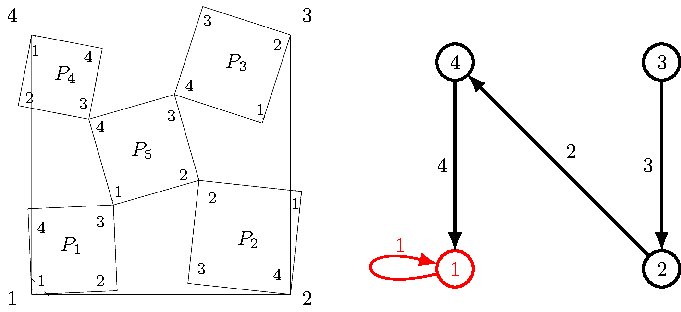
\includegraphics[width=0.7\textwidth]{id2.pdf}
    % \includestandalone[width=0.7\textwidth]{images/tikz1/id2.tex}
    \caption{Всякий путь в индексной диаграмме ведёт в одну из циклических вершин}
    \label{img:id2}
\end{figure}

Пусть $\sa_{AB}=e_1 e_2 e_3 \ldots e_n$ --- путь, направленный из вершины $A$ в $B$, а $\bi=\mu(\sa_{AB}):=i_1\ldots i_n$, где $i_k=\mu(e_k)$. Тогда $A=S_\bi(B)$.

Рассмотрим некоторый бесконечный путь $\sigma=e_1 e_2 e_3 \ldots$, и пусть $A_n=\om(e_n)$. Так как $A=S_{i_1\ldots i_n}(A_n)$, последовательность $\{A_n\}$ называется последовательностью предшественников вершины $A$. Поскольку $A=\lim\limits_{n\to \infty} S_{i_1\ldots i_n}(P)$, то $\mu(\sigma)=i_1\ldots i_n\ldots$ -- адрес точки $A$. Таких адресов может быть несколько.

\begin{figure}[H]
    \centering
    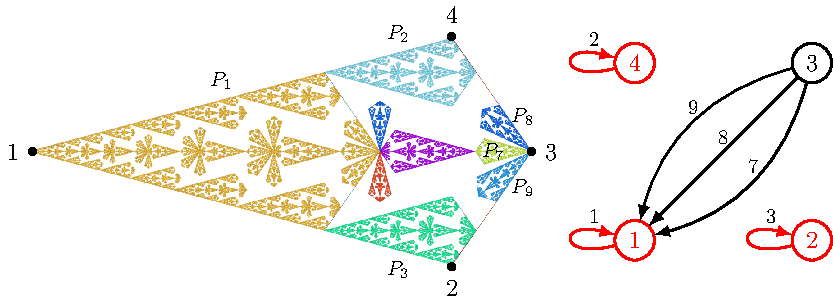
\includegraphics[width=\textwidth]{id3.pdf}
    % \includestandalone[width=\textwidth]{images/tikz1/id3.tex}
\caption{Пример несвязной индексной диаграммы}
\label{img:id3}
\end{figure}

Так как $V_P$ конечно, в последовательности $A, A_1, \ldots, A_n$ найдутся такие $k$ и $l$, что $A_{l}=A_{l+k}$. Тогда $A_{l}=S_{i_{l+1}\ldots i_{l+k}}(A_l)$. В этом случае $A_l$  --- циклическая вершина.

\begin{definition}
Вершина $B\in V_P$ называется циклической, если существует мультииндекс $\bj=j_1\ldots j_k$ такой, что $S_{\bm{j}}(B)=B$. Наименьшая длина $k=|\bj|$ такого мультииндекса называется порядком $B$.
\end{definition}

\begin{figure}[H]
    \centering
    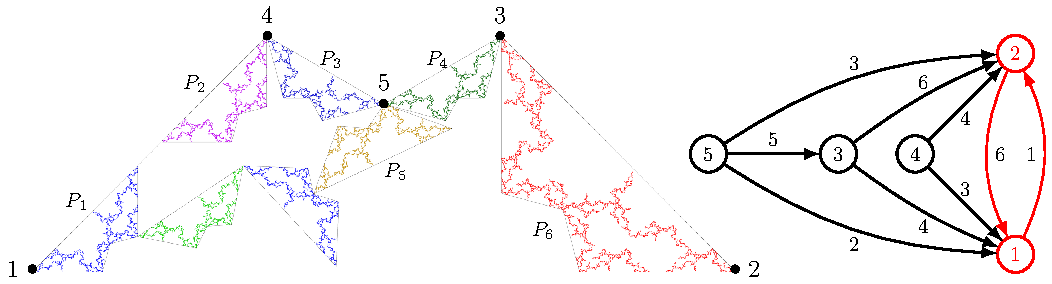
\includegraphics[width=\textwidth]{id4.pdf}
    % \includestandalone[width=\textwidth]{images/tikz1/id4.tex}
    \caption{Пример того, что индексная диаграмма может быть довольно сложной}
    \label{img:id4}
\end{figure}


\begin{definition}
Пусть $A, A_1, A_2, \ldots$ --- последовательность предшественников вершины $A$. 
Говорят, что $A$ подчинена циклической вершине $A_k$, если $A_k$ --- циклическая вершина с наименьшим номером в этой последовательности.
\end{definition}

Таким образом, если $A$ подчинена $A_k$, то для любого $l<k$ точка $A_l=S_{j_1...j_l}^{-1}(A)$ не является циклической вершиной.

\begin{proposition}\label{1ordcyc}
Пусть $\eS$ --- обобщенная $P$-полигональная система подобий.
Всякая вершина $A\in \eV_P$ подчинена некоторой циклической вершине. 
% (2) Существует такой $n$, что в системе $\eS^{(n)}=\{S_\bi, \bi\in I^n\}$ все циклические вершины имеют порядок 1.
\qed 
\end{proposition}

В случае, когда $\eS$ ---  обобщенная полигональная система, условию (1) Теоремы \ref{thm:pcint} и, в частности, когда $\eS$ --- стягиваемая полигональная система,  множество вершин $\eV_P$ и индексная диаграмма $\Ga(\eS)$ имеют следующие свойства: 


\begin{proposition}\label{rankcy}
Пусть  $\eS$ ---  обобщенная полигональная система, удовлетворяющая  условию (1) Теоремы \ref{thm:pcint}, тогда:
\begin{itemize}[nolistsep]
    \item[(i)] в индексной диаграмме $\Ga(\eS)$ все циклические вершины имеют исходящий ранг 1;
    \item[(ii)] всякая циклическая вершина обладает единственным адресом;
    \item[(iii)] существует такое $n$, что все циклические вершины системы $\eS^{(n)}=\{S_\bi,\bi\in I^n\}$ имеют порядок $1$.
\end{itemize}

\end{proposition}

\begin{proof}
Пусть исходящий ранг некоторой циклической вершины $A$ больше 1. 
Это значит что существует циклический путь $\ga$ в $\Ga$ такой что $\al(\ga)=\om(\ga)=A$  и такое ребро $e_1: \al(e_1)=A$, что $e_1\notin\ga$. 
Рассмотрим бесконечный путь $\sigma=e_1 e_2 e_3...$, исходящий из $A$. 
Тогда все пути $\ga^n\sigma$ исходят из $A$ и попарно различны, поэтому $A$ имеет бесконечное множество адресов. 
Поскольку стягиваемая полигональная система является системой с конечным пересечением и удовлетворяет OSC, согласно \cite[Theorem 1.7]{FPS}, множество адресов каждой вершины $P$ конечно. 
Полученное противоречие доказывает (i).
 
Поэтому для всякой циклической вершины $A$ бесконечный путь $\sa$, исходящий из $A$,  единственен, а множество ее предшественников состоит из конечного числа циклических вершин. 
Если выполняется условие (1), $S_i^{-1}A\cap K=S_i^{-1}A\cap \eV_P$, поэтому $\mu(\sa)$ --- единственный адрес точки $A$, что доказывает (ii).\\

Пусть $\Ga$ --- индексная диаграмма системы $\eS$. 
Так как
$\eS^{(n)}$обобщенная полигональная система, удовлетворяющая  условию (1), множество  вершин её индексной диаграммы $\Ga^n$ также есть   $\eV_P$,  а ребрам $e'$ идущим из $A$
в $B$ соответствуют пути $\sa'=e_1...e_n$ длины $n$, такие что $\al(\sa)=A$, $\om(\sa)=B$.
Пусть $n$ --- наименьшее общее кратное порядков всех циклических вершин. 
Для всякого пути $\sa'$ длины $n$, исходящего из циклической вершины $A$, $\om(\sa)=A$. 
Поэтому порядок всякой циклической вершины в системе $\eS^{(n)}$ равен 1.
\end{proof}


\subsection{Структура окрестностей точек в аттракторе стягиваемой полигональной системы.}

1. Пусть  $B\in\eV_P$ --- циклическая вершина стягиваемой полигогальной системы $\eS$. 
Пусть $\bm{j}\in I^*$ --- кратчайший мультииндекс  такой, что $S_{\bm{j}}(B)=B$. 
Тогда подобие $S_{\bm{j}}$ является гомотетией, а угол $\Om_B$, образованный сторонами $P$, прилегающими к $B$, содержит $P$. 
При этом, полагая $W=K\setminus S_{\bm{j}}(K)$ мы получаем представление множества $K$  в виде дизъюнктного объединения 
\begin{equation}\label{wprc}
 K=\{B\}\cup\bigsqcup\limits_{n=0}^\infty S_{\bj}^n(W)   
\end{equation}

\begin{figure}[H]
    \centering
    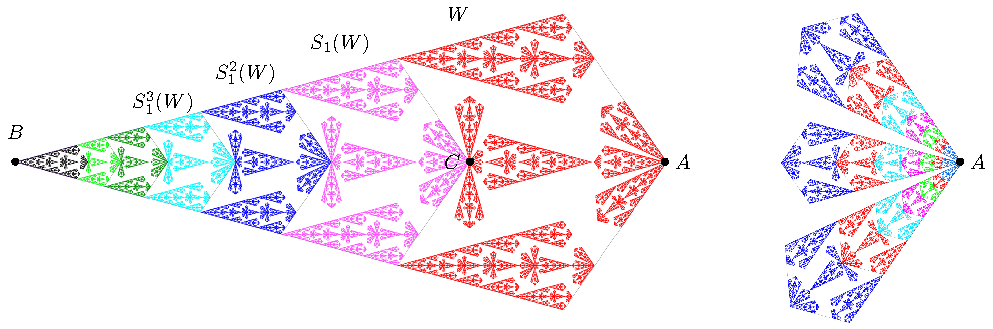
\includegraphics[width=\textwidth]{sot1.pdf}
    % \includestandalone[width=\textwidth]{images/tikz1/sot1.tex}
    \caption{Разбиение \eqref{wprc} аттрактора $K$ в циклической вершине $B$ (слева) и разбиение \eqref{wprnc} стандартной окрестности $U_A$  для нециклической вершины $A$ (справа)}
    \label{img:sot1}
\end{figure}

2. Пусть $A\in V_P$ --- не циклическая вершина. 
Пусть $B_1, \ldots, B_k$ --- полный набор циклических вершин, которым подчинена вершина $A$.
Каждой вершине $B_l$ соответствует такой мультииндекс  $\bi_l$ такой, что $A=S_{\bi_l}(B_l)$ и мультииндекс $\bj_l$ такой, что $S_{\bj_l}(B_l)=B_l$. 
Множества $ S_{\bm{i}_l}(K\setminus B_l)$ попарно не пересекаются и лежат   внутри попарно непересекающихся углов $S_{\bi_l}(\Om_{B_l})$ с общей вершиной $A$. 
При этом множество $U_A=\bigcup\limits_{l=1}^k S_{\bm{i}_l}(K)\cup\{A\}$ является окрестностью вершины $A$ в $K$.Мы назовем ее {\em стандартной окрестностью} вершины $A$.\\
Полагая $W_l=K\mmm S_{\bj_l}(K)$, мы получаем представление стандартной окрестности вершины $A$ в виде:
\begin{equation} \label{wprnc} 
U_A=\{A\}\cup\bigsqcup\limits_{l=1}^k S_{\bi_l}\bigsqcup\limits_{n=0}^\infty S_{\bj_l}^n(W_l)
\end{equation}

3. Рассмотрим точку $A\in G_\eS (\eV_P)$. 
Для нее также можно определить её стандартную окрестность $U_A$ в $K$.

\begin{definition}
Будем говорить, что $A\in G_\eS (\eV_P)$ подчинена циклической вершине $B$, если $A=S_{j_1...j_k}(B)$ и
 для любого $l<k$ точка $S_{j_1...j_l}^{-1}(A)$ не является циклической вершиной. 
\end{definition}

\begin{figure}[H]
    \centering
    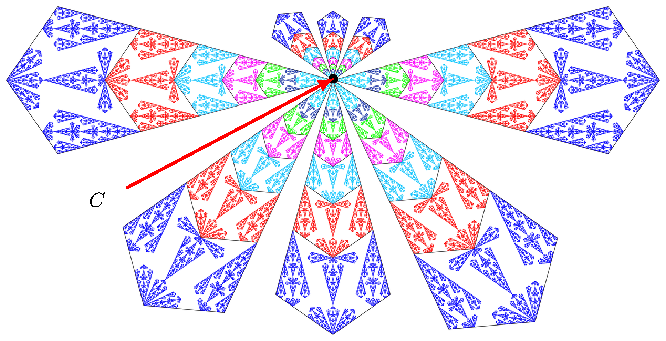
\includegraphics{sot2.pdf}
    % \includestandalone{images/tikz1/sot2.tex}
    \caption{Разбиение \eqref{wprnc} стандартной окрестности $U_C$  для точки $C\in G_\eS (\eV_P)$}
    \label{img:sot2}
\end{figure}

Учитывая свойства многоугольников $P_\bj$ и структуру окрестностей вершин $P_\bj$, мы приходим к выводу, что для каждой точки $A\in G_\eS (V_P)$ также существует полный набор циклических вершин $B_1, \ldots, B_k$, которым подчинена точка $A$ и соответствующие наборы мультииндексов $\bi_l, \bj_l$, задающие  стандартную окрестность $U_A$ и её представление \eqref{wprnc}.





% \begin{theorem}%\label{refsys} 
% Пусть $\eS$ --- это стягиваемая $P$-полигональная система подобий.
% Тогда для любого $x\in G_\eS(\eV_P)$ существует $\ep>0$ и конечная система $\{\Om_1,...,\Om_n\} ($ где $n=\#\pi^{-1}(x)$) непересекающихся углов с вершиной  $x$, таких, что если $x\in P_\bj$ и $\diam P_\bj<\ep$, то для некоторых $k\le n$, $\Om(P_\bj,x)=\Om_k$. 
% И наоборот, для любого $\Om_k$ существует такой $\bj\in\ia$, что  $\Om(P_\bj,x)=\Om_k$.
% \end{theorem}

\subsection{Теорема о совпадении параметров.}

Пусть $A$ --- циклическая вершина обобщенной $P$-полигональной системы $\eS$. 
В этом случае отображение $S_\bi$, для которого $S_\bi(A)=A$, не обязательно является гомотетией, и тогда мы должны определить угол поворота  такого отображения. 
Формально угол поворота $\al_i$ отображения $S_\bi$ определяется с точностью до $2n\pi$, но в случае полигональных систем число $n$ однозначно определяется системой многоугольников $\wP$ и зависит от геометрической конфигурации этой системы.



\begin{proposition}\label{fixparc}
Пусть $\eS$ -- обобщенная $P$-полигональная система, удовлетворяющая условию (\ref{icnd}), и пусть $A$ --- циклическая вершина многоугольника $P$. 
Тогда существуют такая вершина $B\in V_{P}$ и такой мультииндекс $\bi\in \ia$, что  $S_{\bi}(A)=A$  и жорданова дуга $\ga_{AB}\IN K$ удовлетворяет включению $S_{\bi}(\ga_{AB})\IN\ga_{AB}$.
\end{proposition}

\begin{proof}
Пусть $\bj$ --- кратчайший из мультииндексов, для которого $A=S_\bj(A)$. 
Пусть $W=K\mmm S_\bj(K)$, тогда 
$$K=\{A\}\cup\bigsqcup\limits_{n=0}^\infty S_{\bj}^n(W).$$
Пусть $Q=S_\bj^{-1}(\bar W\cap S_\bj(K))$. 
Исходя из Замечания \ref{fpro}, мы видим, что $Q\IN\eV\mmm \{A\}$. 

Вершина $A$ не может принадлежать $Q$.
В противном случае существовала бы копия $K_\bi$ такая что $K_\bi\cap K_\bj=\{A\}$, а для любых $k,l$, $S_\bj^k(K_\bi)\cap S_\bj^l(K_\bi)=\{A\}$. 
В этом случае $A$ была бы точкой ветвления бесконечного порядка в $K$, что невозможно по Теореме \ref{thm:pcint}.\\
 
Так как  $K$ --- дендрит, для каждой точки $B\in Q$ существует единственная дуга $\ga_{AB}\IN K$. Пусть $\ga_{B'B}$ --- наименьшая из ее поддуг таких, что $B'\in K_\bj$. Тогда $B'\in S_\bj(Q)$. 
Зададим отображение $\psi:Q\to Q$ формулой $\psi(B)=S_\bj^{-1}(B')$. 
Тогда для любого $B\in Q$, $S_\bj(\ga_{A\psi(B)})\IN \ga_{AB}$. Далее, для любого $n$, $S^n_\bj(\ga_{A\psi^n(B)})\IN \ga_{AB}$.

Так как $\psi$ --- отображение конечного множества $Q$ в себя, существуют такие $n$ и $B\in Q$, что $\psi^n(B)=B$. 
Тогда $S_\bj^n(\ga_{AB})\IN\ga_{AB}$.
Положим $S_\bi=S_\bj^n$.
\end{proof}

\begin{definition} 
Дуга $\ga_{AB}$ называется {\em инвариантной дугой} циклической вершины $A$.
\end{definition}

Пусть $A$ -- циклическая вершина, $\ga_{AB}$ -- её инвариантная дуга, и $S_\bi(A)=A$. 
Пусть $B'=S_\bi(B)$. 
Обозначим через $\al$ совокупное изменение аргумента $z-A$ при перемещении $z$ по $\ga_{AB}$ от $B$ до $B'$. 
Это дает нам единственное представление  $S_\bi(z)=q_\bi e^{i\al}(z-A)+A$. 

\begin{remark} 
На следующем Рисунке показано, как угол $\al$ зависит от геометрической конфигурации системы $\eS$, хотя одно и то же подобие фиксирует $A$ и отображает $B$ в $B'$.
\end{remark}

\begin{figure}[H]
    \centering
    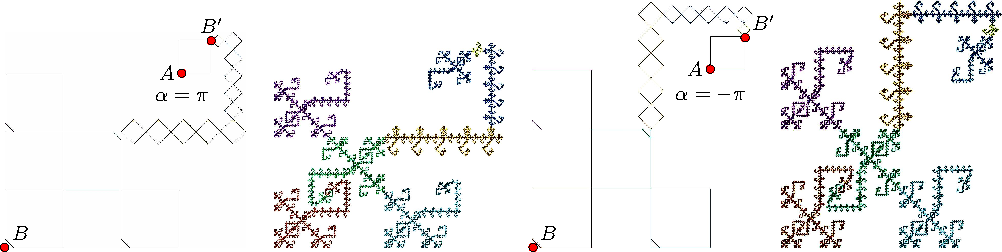
\includegraphics[width=\textwidth]{superden.pdf}
    % \includestandalone[width=\textwidth]{images/tikz1/superden.tex}
    \caption{}
    \label{img:superden}
\end{figure}

\begin{definition}
Число $\lambda_A=\dfrac{\al}{\ln{r}}$ называется параметром циклической вершины $A$.
\end{definition}

\begin{definition}
Обобщенная $P$-полигональная система $\eS$ подобий удовлетворяет {\em условию совпадения параметров}, если для любого $B \in\cup_{i=1}^m  \eV_{P_i}$ и для любых циклических вершин $A,A'$  таких, что для некоторых $\bi,\bj\in I^*$,  $S_\bi(A)=S_\bj(A')=B$, выполняется равенство $\lambda _{A}=\lambda _{A'}$.
\end{definition}

% \red{
% Поскольку у вершин, находящимся в одном цикле индексной диаграммы или же подчиненным такому циклу, совпадают параметры, то это является большим подспорьем при проектировании обобщенных полигональных систем. В противном случае, если не пользоваться этим свойством циклических вершин, то остается только подгонять вручную размеры и повороты подобий так, чтобы их параметры совпадали.}

Из Предложений \ref{1ordcyc} и \ref{fixparc}, и Леммы В.В. Асеева о непересекающихся периодических дугах \cite[Lemma 3.1]{ATK} Мы приходим к следующей Теореме о совпадении параметров:

\begin{theorem}\label{PMT}
Пусть обобщенная $P'$-полигональная система $\eS'$ является  $\da$-деформацией стягиваемой $P$-полигональной системы  $\eS$, а аттрактор $K'$ системы $\eS'$ является дендритом. 
Тогда система $\eS'$ удовлетворяет условию совпадения параметров.
\end{theorem}

\begin{proof}
Пусть $\eS$ --- обобщенная полигональная система, аттрактор $K$ которой --- дендрит. 
Пусть $C \in\cup_{i=1}^m  \eV_{P_i}$ и $A,A'\in \eV_P$ --- такие циклические вершины, что для некоторых $i,j\in I$  $S_i(A)=S_j(A')=C$. 
Обозначим образы $S_i(K)$ и $S_j(K)$ как $K_i,\ K_j$ соответственно. 
Без потери общности можно допустить, что точка $C$ имеет координату $0$ в $\bbc$. 
Поскольку для некоторых $\bi,\bj\in I^*$, $S_\bi(A)=A$ и $S_\bj(A')=A'$, отображения $S_{b1}=S_iS_\bi S_i^{-1}$ и $S_{b2}=S_jS_\bj S_j^{-1}$ имеют $C$  в качестве своей неподвижной точки, а $S_{b1}(K_i)\IN K_i$ и $S_{b2}(K_j)\IN K_j$. 
Пусть $S_{b1}(z)=q_\bi e^{i\al_\bi}z$ и $S_{b2}(z)=q_\bj e^{i\al_\bj}z$. 
Так параметрами вершин $A$ и $A'$ будут $\la_1=\dfrac{\al_\bi}{\log q_\bi}$ и  $\la_2=\dfrac{\al_\bj}{\log q_\bj}$. 
Пусть $\ga_{AB}\IN K$ и $\ga_{A'B'}\IN K$ являются инвариантными дугами для вершин $A$ и $A'$. 
Пусть также  $\ga_1=S_i(\ga_{AB})$ и $\ga_2=S_j(\ga_{A'B'})$. 
Тогда $S_{b1}(\ga_1)\IN \ga_1$ и $S_{b2}(\ga_2)\IN \ga_2$. 
По Лемме В.В. Асеева о непересекающихся периодических дугах \cite[Lemma 3.1]{ATK} следует, что если $\ga_1\cap\ga_2=\{C\}$, то $\la_1=\la_2$.
\end{proof}

Технически, теорема о совпадении параметров показывает необходимое условие того, что аттрактор $\da$-деформации будет дендритом. 
Однако если стягиваемую полигональную систему деформировать слишком сильно, то даже при соблюдении условия совпадения параметров аттрактор $\da$-деформации может и не быть дендритом. 
Значит нам нужны ограничения при деформациях. 
Поэтому далее мы оценим $\da$ в доказательстве теоремы о малых деформациях. 
Эта оценка и будет представлять из себя достаточное условие того, что аттрактор $\da$-деформации будет дендритом.



\newpage
\section{Теорема о малых деформациях}

\subsection{Основные параметры стягиваемой полигональной системы}\label{parms}

Для любого множества $X\IN\rr^2$ или точки $A$ через $V_\ep(X)$ (соотв.$V_\ep(A)$) мы обозначаем $\ep$-окрестности множества $X$ (соотв. точки $A$) на плоскости.\\

{\bf Параметр  $\bm{\rho_0:}$}   Обозначим через $\rho_0>0$, наименьшее из попарных расстояний между точками непересекающихся многоугольников $P_i,P_j$ и  расстояний от вершин $A\in\eV_p$ до точек многоугольников $P_i\not\ni A$:
\begin{itemize}[nolistsep]
    \item[(i)] для любой вершины $A\in \eV_P$,   $V_\rho(A) \bigcap P_k \ne \0 \Rightarrow A\in P_k$;
    \item[(ii)] для любых $x, y \in P$, для которых существуют такие $P_k, P_l$, что $x \in P_k, y \in P_l$ и $P_k \bigcap P_l = \0$, выполняется $d (x, y) \ge \rho_0$.
\end{itemize}

\begin{figure}[H]
    \centering
    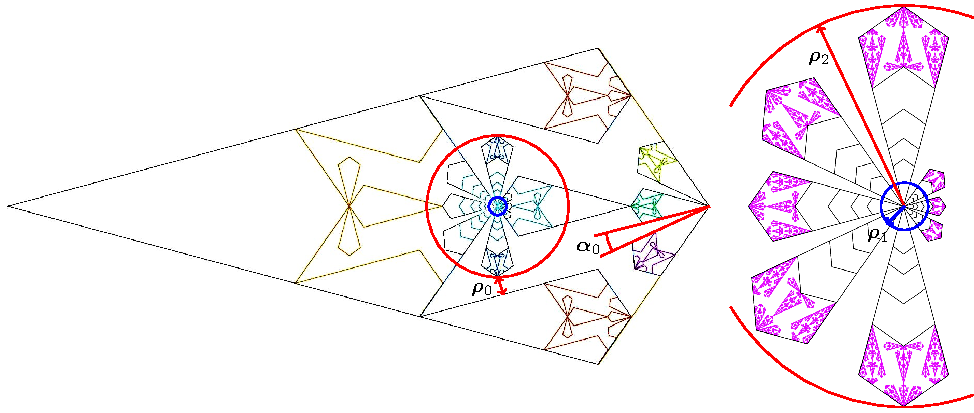
\includegraphics{par1.pdf}
    % \includestandalone{images/tikz1/par1.tex}
    \caption{Выбор параметров $\al_0$, $\rho_0$, $\rho_1$ и $\rho_2$ для полигональной системы}
    \label{img:par1}
\end{figure}

{\bf Параметры  $\bm{\rho_1,\rho_2:}$}  Пусть $C\in\eV_{\tilde P}$ --- не циклическая точка. 
Пусть $U_C$ --- ее стандартная окрестность, а  $\tilde U_C=\bigcup\limits_{l=1}^k S_{\bi_l}(W_l)$. 
Тогда $\rho_1$ и $\rho_2$ выбираются такими, что для любого $C\in\eV_{\tilde P}$, множество $\tilde U_C$ содержится в кольце $\rho_1<|z-C|\le\rho_2$.


{\bf Параметр $\bm{\al_0:}$} $\al_0$ --- наименьший возможный угол между теми сторонами многоугольников $P_i, P_j, i,j\in I$, которые имеют общую вершину.\\
  
{\bf Обозначения для отображений  циклических вершин.} 
В случае, когда $\eS$ --- стягиваемая $P$-полигональная система, все циклические вершины которой имеют порядок 1, мы  упорядочим индексы в $I$ и пронумеруем вершины в $\eV_P$ таким образом, что каждой циклической вершине $A_l$ соответствует гомотетия $S_l(z)=q_l(z-A_l)+A_l$. 
При этом $K$  лежит внутри угла $\Om(P, A_l)$ и $K\mmm \{A_l\} =\bigsqcup\limits_{n=0}^\8S_l^n(W_l)$. 



\subsection{Оценка $\da$ и главная теорема}

{\bf Исходные предположения.} 
Пусть $\eS=\{S_1,...,S_m\}$ -- стягиваемая $P$-полигональная система, а отображение $f$ задает $\da$-деформацию системы $\eS$ в обобщенную $P'$-полигональную систему $\eS'=\{S'_1,...,S'_m\}$, где $S_k(z)=q_k e^{i\al_k}(z-z_k)+z_k$ и $S'_k(z)=q'_k e^{i\al'_k}(z-z'_k)+z'_k$.\\ 
Мы  предполагаем, что $\diam P=1$, а $\da>0$ таково, что 
\begin{equation}\label{assum}
\da<q_{min}/8\quad\text{ и }\quad\da<(1-q_{max})/8
\end{equation}

Получим оценки изменения $\Da q_k=|q'_k-q_k|$ и $\Da \al_k=|\al'_k-\al_k|$ при деформации $f$:

\begin{lemma}\label{lasin}
Для  любого $k\in I$,
\begin{equation}\label{dadq}
\Da q_k<3\da  \mbox{\quad и \quad} \Da \al_k< 
C_\al\da \mbox{, где }C_\al=2.1(1+1/q_{min})
\end{equation}
\end{lemma} 

\begin{proof}
Выберем такие вершины $A,B$   многоугольника $P$, что $|B-A|=1$. 
Используем для образов  $A$ обозначения $A_k=S_k(A)$, $A'=f(A)$ и $A'_k=f(A_k)=S'_k(A')$, и аналогичные -- для  вершины $B$.\\ 
Оценим изменение модуля и аргумента для $\dfrac{B_k-A_k}{B-A}=q_k e^{i\al_k}$ и $\dfrac{B'_k-A'_k}{B'-A'}=q'_k e^{i\al'_k}$.\\

Так как $f$ -- $\da$-деформация,  $|(B_k-A_k)|-2\da\le|(B'_k-A'_k)|\le |(B_k-A_k)|+2\da$. Это влечет 
\begin{equation}\label{dmod}
3q_{min}/5<\dfrac{q_{min}-2\da}{1+2\da}<\dfrac{q_k-2\da}{1+2\da}\le q'_k\le \dfrac{q_k+2\da}{1-2\da}<\dfrac{q_{max}+2\da}{1-2\da}<\dfrac{1+3q_{max}}{3+q_{max}}.
\end{equation}
Так как
\begin{equation}\label{dal}
\al'_i-\al_i
%=\arg\dfrac{B'_k-A_k'}{B'-A'}\dfrac{B-A}{B_k-A_k}
=\arg\dfrac{B'_k-A_k'}{B_k-A_k}-\arg\dfrac{B'-A'}{B-A},
\end{equation}
мы получаем 
\begin{equation}\label{darg}
|\al_k'-\al_k|\le \arcsin 2\da+\arcsin \dfrac{2\da}{q_k}
\end{equation}

Подставляя неравенства \eqref{assum}  в \eqref{dmod} и \eqref{darg} и учитывая,  что если $0<x<0.5$, то $0<\arcsin x<1.05x$,
% в соответствии с допущениями (\ref{assum}), $3q_{min}/5<\dfrac{q_{min}-2\da}{1+2\da}<q'_k<\dfrac{q_{max}+2\da}{1-2\da}<\dfrac{1+3q_{max}}{3+q_{max}}$;\\ 
% принимая во внимание то, что $q_k<1$ и $1-2\da>3/4$, и что если $0<x<.5$, то $\arcsin x<1.05x$, 
мы получаем оценки
\begin{equation}\label{dadq1}
\Da q_k=|q'_k-q_k|<\dfrac{2\da(1+q_k)}{1-2\da}<3\da  \mbox{\quad и \quad} \Da \al_k=|\al'_k-\al_k|< C_\al\da ,
\end{equation} 
где $C_\al=2.1(1+1/q_{min})$.
\end{proof}

Пусть $V_\da(P)$ обозначает $\da$-окрестность многоугольника $P$.

\begin{lemma}\label{vda1}
Пусть $\da_1=\dfrac{4\da}{1-q_{max}}$, а  $U=V_{\da_1}(P)$. Тогда:
\begin{itemize}[nolistsep]
    \item[(1)] для любого $k\in I$,\  $S_k(U)\IN U$ и $S'_k(U)\IN U$;
    \item[(2)] для любого $z\in U$, $|S'_k(z)-S_k(z)|<C_\Da\da$, где $C_\Da=6.5+1.5C_\al$.
\end{itemize}
\end{lemma} 


\begin{proof}
(1) По Определению \ref{dfn:deform}, $V_\da(P_k)\NI P'_k$, $V_\da(P'_k)\NI P_k$, 
$V_\da(P)\NI P'$ и $V_\da(P')\NI P$.\\

Таким образом,  $S_k'(P')\IN V_\da(P_k)\IN V_\da(P)$. Поэтому
$S_k'(P)\IN V_{2\da}(P_k)\IN V_{2\da}(P)$.\\


Так как $S_k'$ --- подобие, $S_k'(V_\rho(P))\IN V_{2\da+q'_k\rho}(P)$ для любого положительного $\rho$.

Если $\rho\ge\dfrac{2\da}{1-q_k'}$, то  $2\da+q'_k\rho\le \rho$,  поэтому $S_k'(V_{\rho}(P))\IN V_{\rho}(P)$.\\ Из неравенств $q_k'< \dfrac{q_{max} +2\da}{1-2\da}
$  следует $\dfrac{2\da}{1-q_k'}\le\dfrac{2\da(1-2\da)}{1-q_{max}-4\da}<\dfrac{4\da}{1-q_{max}}$, а это влечет (1). При этом, в силу  \eqref{assum}, $\da_1< 1/2$.\\  


(2) Возьмем $z\in U$ и оценим разность $S'_k(z)-S_k(z)$. Её можно представить в виде $S'_k(A)-S_k(A)+(q'_ke^{i\al'_k}-q_ke^{i\al_k})(z-A)$. Поэтому 
\begin{equation}\label{delta}
|S'_k(z)-S_k(z)|<|S'_k(A)-S_k(A)|+(|q'_k-q_k|+q_k|e^{i\al'_k}-e^{i\al_k}|)|z-A|.
\end{equation} 
Так как $|z-A|<1+\da_1<1.5$, $|S'_k(A)-S_k(A)|<2\da$, a $|e^{i\al'_k}-e^{i\al_k}|\le |\al'_k-\al_k|$, правая часть неравенства (\ref{delta}) не превышает $2\da+1.5(3\da+C_\al\da)$.
\end{proof}


Применяя к $\eS,\eS'$ и $U$ Теорему о смещении \cite[Theorem 17]{TF}, получаем
\begin{proposition}\label{deltaK}
Пусть $\pi,\pi'$ -- индексные отображения для систем $\eS$ и $\eS'$.\\
1. Для любого $\sa\in I^\8$, 
\begin{equation}\label{dKeq} 
|\pi'(\sa)-\pi(\sa)|< C_K\da \mbox{   где   }C_K=\dfrac{C_\Da}{1-q_{max}}
\end{equation} 
2. Если система $\eS^{'(n)}$ удовлетворяет  {\bf D2--D4}, то она является $(C_K\da)$-деформацией системы $\eS^{(n)}$.
\qed
\end{proposition}

\begin{remark}\label{Sshift}
Пусть  $\eS'=\{S'_1,...,S'_m\}$ --- это  $\da$-деформация стягиваемой $P$-полигональной системы $\eS$. Пусть $A\in S_j(\eV_P)$ для некоторого $j\in I$. Пусть $g(z)=z-A+A'$ и $\hat S''_k=g\circ S'_k\circ g^{-1}$.
Тогда $\eS''=\{S''_1,...,S''_m\}$ является $2\da$-деформацией системы $\eS$, для которой $A''=A$, $K''=g(K')$, $P''_\bj=g(P_\bj)$. Поскольку $g$ -- это сдвиг, оценки (\ref{lasin}) и (\ref{dadq}) для $\eS''$ остаются неизменными с тем же $\da$, в то время как $|\pi''(\sa)-\pi(\sa)|< (C_K+1)\da$. Таким образом мы обозначаем  $\da_2=(C_K+1)\da$.
\end{remark}

Принимая во внимание Предложения \ref{1ordcyc} и \ref{deltaK}, достаточно доказать теорему для случая, когда все циклические вершины системы $\eS$ имеют порядок 1.

\begin{proposition}
Пусть выполнены Исходные предположения, а  $S_k(z)=q_k(z-A_k)+A_k$ -- гомотетия, переводящая в себя $A_k\in \eV_P$.  Тогда  параметр $\la_k$  отображения  $S'_k$  удовлетворяет неравенству
\begin{equation}\label{prmeq2}
|\la_k|<C_\la\da\mbox{, где }C_\la=\dfrac{2.1(1+1/q_{max})}{\log(3+q_{max})-\log(3q_{max}+1)}.
\end{equation}
\end{proposition}

\begin{proof}
Из \ref{lasin} следует, что
\begin{equation}\label{parmeq}
|\la_k|\le\dfrac{\arcsin 2\da+\arcsin\dfrac{2\da}{q_k}}{|\log(q_k+2\da)-\log(1-2\da)|}
\end{equation}

Учитывая неравенства \eqref{dmod} и \eqref{darg}, получаем \eqref{prmeq2}.
\end{proof}



\begin{lemma}
Пусть $\eS$ -- стягиваемая $P$-полигональная система, циклические вершины котрой имеют порядок 1, а $\eS'$ -- её $\da$-деформация. Тогда если 
\begin{equation} \label{mineq}
2.1\dfrac{\da_2}{\rho_1}+\la\log\dfrac{\rho_2+\da_2}{\rho_1-\da_2}<\al_0 \mbox{ и }  2\da_2<\rho_0,
\end{equation} 
то система $\eS'$ удовлетворяет Условию (\ref{icnd})
\end{lemma}  
 
 
\begin{remark}\label{logs} 
Если предположить, что $\da_2<\rho_1/4$, а $\da_2<(1-\rho_2)/4$, то неравенство \eqref{mineq} сследует из
 \[2.1\dfrac{\da_2}{\rho_1}+\la\log\dfrac{1+3\rho_2}{3\rho_1}<\al_0\]
\end{remark} 
   

\begin{proof}
Возьмем вершину $B\in V_\wP$.  Учитывая Замечание \ref{Sshift}, мы можем предположить, что $B=0$ и $f(0)=0$, поэтому $B'=B=0$.

Разложение  стандартной окрестности $U_B$ точки $B$ имеет вид
\begin{equation} \label{wprx} 
U_B=\{B\}\cup\bigsqcup\limits_{l=1}^k S_{\bj_l}\bigsqcup\limits_{n=0}^\infty S_l^n(W_l)
\end{equation}

 Отображения $\bar S_l=S_{\bj_l}S_{i_l}S_{\bj_l}^{-1}$ являются гомотетиями с неподвижной точкой $B$, такими что 
\begin{equation}\label{kbj} 
K_{\bj_l}\mmm\{B\}=\bigsqcup\limits_{n=0}^\8\bar S_l^n(W_l)
\end{equation} 
Аналогично, пусть $W'_l=\hat f(W_l)$ и $\bar S'_l=S'_{\bj_l}S'_{i_l}S_{\bj_l}^{'-1}$. Тогда
\begin{equation} \label{kpbj} 
K'_{\bj_l}\mmm\{B\}=\bigsqcup\limits_{n=0}^\8\bar S_l^{'n}(W'_l)
\end{equation}
Заметим, что  $\bar S_l(z)=q_{i_l}z$ и $\bar S'_l(z)=q'_{i_l}e^{i\al_{i_l}}z$ для любого $l$, а из за условия совпадения параметров существует такой  $\la$, что для любого $l$ $\al_{i_l}=\la\log q'_{i_l}$. 
  
Рассмотрим отображение $z = exp(w)$ плоскости $(w = \ro+i\fy)$ как универсальное покрытие проколотой плоскости $\bbc\mmm\{0\}$. 

Рассмотрим многоугольники $P_{\bj_l}$ и выберем их поднятия на плоскости $(w = \ro+i\fy)$.
Мы можем предположить, что эти поднятия лежат в соответствующих горизонтальных полосах $\te^-_l\le\fy\le\te^+_l$, где $0<\te^-_l<\te^+_l<2\pi$ и $\te^+_l+\al_0<\te^-_{l+1}$ для любого $l<k$, и $\te^+_k+\al_0<\te^-_1 +2\pi$.
Мы также рассматриваем поднятия множеств $K_{\bj_l}$, $W_l$, $K'_{\bj_l}$ и
$W'_l$. Обозначим эти поднятия как $\eK_{\bj_l}$, $\eW_l$, $\eK'_{\bj_l}$ и
$\eW'_l$.
Из уравнений \ref{kbj} и \ref{kpbj} следует, что
\begin{equation}\label{ekbj} 
\eK_{\bj_l}
    =\bigsqcup\limits_{n=0}^\8\bar T_l^n(\eW_l) \mbox{\quad и \quad} \eK'_{\bj_l}
    =\bigsqcup\limits_{n=0}^\8\bar T_l^{'n}(\eW'_l), 
\end{equation}  
где $T_l(w)=w+\log q_l$   и   $T'_l(w)=w+(1+i\la)\log q'_l$ являются параллельными переносами, для которых $T_l(\eK_l)\IN \eK_l$ и $T'_l(\eK'_l)\IN \eK'_l$.

\begin{figure}[H]
    \centering
    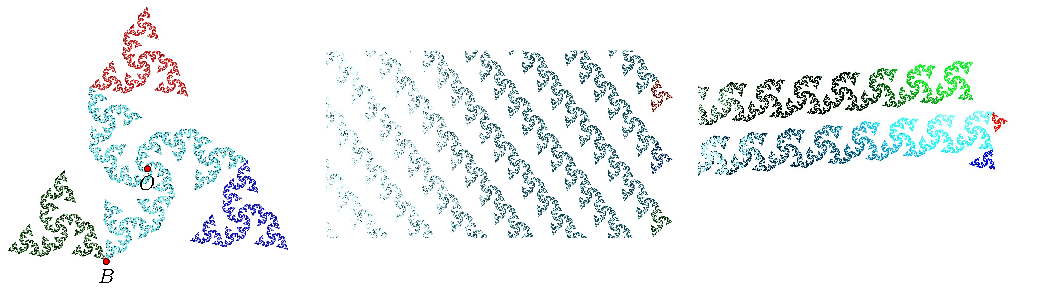
\includegraphics[width=\textwidth]{log.pdf}
    % \includestandalone[width=\textwidth]{images/tikz1/log.tex}
    \caption{Образы множества $K'$ относительно отбражения $w=\log(z-O)$ и отображения $w=\log(z-B)$.}
    \label{img:log}
\end{figure}

Множества $\eK_l$ лежат в полуполосах $ \ro\le \log\rho_2, \te^-_l\le\fy\le\te^+_l$, в то время как множества $\eW_l$ содержатся в прямоугольниках $R_l=\{\log\rho_1 \le\ro\le \log\rho_2, \te^-_l\le\fy\le\te^+_l\}$.

Тогда множества $\eW'_l$ лежат в прямоугольнике 
\begin{equation} 
R'_l=\left\{\log(\rho_1-\da_2)\le\ro\le \log(\rho_2+\da_2), \te^-_l-1.05\dfrac{\da_2}{\rho_1}\le\fy\le\te^+_l+1.05\dfrac{\da_2}{\rho_1}\right\}
\end{equation}

Каждое объединение  $\bigcup\limits_{n=0}^\8T^{'n}_l(R'_l)$ лежит в полуполосе 
\begin{equation} 
\begin{cases}
\ro\le \log(\rho_2+\da_2)\\   
\te^-_l-1.05\dfrac{\da_2}{\rho_1}-\la \log(\rho_2+\da_2)\le\fy-\la\ro\le \te^+_l+1.05\dfrac{\da_2}{\rho_1}-\la \log(\rho_1-\da_2)
\end{cases}
\end{equation}

Поэтому множество $\eK'_{\bj_l}$ тоже лежит в этой полуполосе.
Тогда если 
\begin{equation}
\te^+_{l-1}+1.05\dfrac{\da_2}{\rho_1}-\la \log(\rho_1-\da_2)<\te^-_l-1.05\dfrac{\da_2}{\rho_1}-\la \log(\rho_2+\da_2),
\end{equation} 
то $\eK'_{\bj_{l-1}}\cap\eK'_{\bj_l}=\0$.

Мы можем гарантировать, что такое неравенство справедливо для любого $l$, если 
$2.1\dfrac{\da_2}{\rho_1}+\la\log\dfrac{\rho_2+\da_2}{\rho_1-\da_2}<\al_0$.

Если, кроме того, $2\da_2<\rho_0$, то для любоых $i_1,i_2\in I$  таких что $P_{i_1}\cap P_{i_2}=\0$, $P'_{i_1}\cap P'_{i_2}=\0$  и $K'_{i_1}\cap K'_{i_2}=\0$ откуда следует условие (\ref{icnd}).
\end{proof}
 
 
\begin{theorem}\label{mainthm}
Пусть $\eS$ -- стягиваемая $P$-полигональная система. Существует такое $\da>0$, что для любой $\da$-деформации $\eS'$ системы $\eS$, удовлетворяющей условию совпадения параметров, аттрактор $K(\eS')$ будет дендритом, гомеоморфным $K(\eS)$.
\end{theorem}

\begin{proof}
Пусть все циклические вершины $P$-полигональной системы $\eS$ имеют порядок 1. 
Если мы   скомбинируем неравенства \ref{dadq}, \ref{dKeq}, \ref{prmeq2}, \ref{mineq} с учетом Замечания \ref{logs}, мы увидим, что, если выполняются следующие неравенства:\\
1. $\da<\dfrac{\min(q_{min},1-q_{max})}{8}$;\qquad\qquad
2. $\da<\dfrac{\min(\rho_0,\rho_1,1-\rho_2)}{2(C_K+1)}$;\\
 и  
3. $\da<\dfrac{\al_0}{\dfrac{2.1(C_K+1)}{\rho_1}+C_\la\log\dfrac{1+3\rho_2}{3\rho_1}}$,\\ 
то аттрактор $K'$ $\da$-деформации $\eS'$ системы $\eS$ удовлетворяет условию (\ref{icnd}). 
Следовательно $K'$ -- дендрит. 
По Теореме \ref{thm:attrmap}, отображение $\hat f:K\to K'$ биективно, и следовательно оно является гомеоморфизмом.
 
Предположим теперь, что $\eS$ имеет циклические вершины порядка больше $1$, и пусть $M=12+4.2\left(1+\dfrac{1}{q_{min}}\right)$. 
Существует такое $n$, что система $\eS^{(n)}$ имеет циклические вершины порядка $1$. 
Предположим, что любая $\da$-деформация системы $\eS^{(n)}$ порождает дендрит. 
Тогда для любой $\da/M$-деформации $\eS'$ системы $\eS$, система $\eS^{'(n)}$ будет $\da$-деформацией системы $\eS^{(n)}$.
\end{proof}